\documentclass[12pt,oneside]{uhthesis}
\usepackage{subfigure}
\usepackage[ruled,lined,linesnumbered,titlenumbered,algochapter,spanish,onelanguage]{algorithm2e}
\usepackage{amsmath}
\usepackage{amssymb}
\usepackage{amsbsy}
\usepackage{caption,booktabs}
\captionsetup{ justification = centering }
%\usepackage{mathpazo}
\usepackage{float}
\setlength{\marginparwidth}{2cm}
\usepackage{todonotes}
\usepackage{listings}
\usepackage{xcolor}
\usepackage{multicol}
\usepackage{graphicx}
\floatstyle{plaintop}
\restylefloat{table}
\addbibresource{Bibliography.bib}
% \setlength{\parskip}{\baselineskip}%
\renewcommand{\tablename}{Tabla}
\renewcommand{\listalgorithmcfname}{Índice de Algoritmos}
%\dontprintsemicolon
\SetAlgoNoEnd

\definecolor{codegreen}{rgb}{0,0.6,0}
\definecolor{codegray}{rgb}{0.5,0.5,0.5}
\definecolor{codepurple}{rgb}{0.58,0,0.82}
\definecolor{backcolour}{rgb}{0.95,0.95,0.92}

\lstdefinestyle{mystyle}{
    backgroundcolor=\color{backcolour},   
    commentstyle=\color{codegreen},
    keywordstyle=\color{purple},
    numberstyle=\tiny\color{codegray},
    stringstyle=\color{codepurple},
    basicstyle=\ttfamily\footnotesize,
    breakatwhitespace=false,         
    breaklines=true,                 
    captionpos=b,                    
    keepspaces=true,                 
    numbers=left,                    
    numbersep=5pt,                  
    showspaces=false,                
    showstringspaces=false,
    showtabs=false,                  
    tabsize=4
}

\lstset{style=mystyle}

\title{Detecci\'on de patrones en im\'agenes de mamograf\'ias digitales}
\author{\\\vspace{0.25cm}Miguel Alejandro Asin Barthelemy}
\advisor{\\\vspace{0.25cm}MSc. Damian Valdés Santiago}
\degree{Licenciado en (Matemática o Ciencia de la Computación)}
\faculty{Facultad de Matemática y Computación}
\date{28 de Diciembre de 2022\\\vspace{0.25cm}\href{https://github.com/M4S1N/thesis}{github.com/M4S1N/thesis}}
\logo{Graphics/uhlogo}
\makenomenclature

\renewcommand{\vec}[1]{\boldsymbol{#1}}
\newcommand{\diff}[1]{\ensuremath{\mathrm{d}#1}}
\newcommand{\me}[1]{\mathrm{e}^{#1}}
\newcommand{\pf}{\mathfrak{p}}
\newcommand{\qf}{\mathfrak{q}}
%\newcommand{\kf}{\mathfrak{k}}
\newcommand{\kt}{\mathtt{k}}
\newcommand{\mf}{\mathfrak{m}}
\newcommand{\hf}{\mathfrak{h}}
\newcommand{\fac}{\mathrm{fac}}
\newcommand{\maxx}[1]{\max\left\{ #1 \right\} }
\newcommand{\minn}[1]{\min\left\{ #1 \right\} }
\newcommand{\lldpcf}{1.25}
\newcommand{\nnorm}[1]{\left\lvert #1 \right\rvert }
\renewcommand{\lstlistingname}{Ejemplo de código}
\renewcommand{\lstlistlistingname}{Ejemplos de código}

\begin{document}

\frontmatter
\maketitle

\begin{dedication}
	\textit{Dedico este logro a la persona que me ha dado la fuerza para seguir adelante pese a todos los tropiezos.}
\end{dedication}
\begin{acknowledgements}
    \par A mi familia por apoyarme en todo momento.
    \par A mis compa\~neros por los buenos y malos momentos que pasamos juntos.
    \par A mi tutor Dami\'an por creer en que lo pod\'ia lograr.
\end{acknowledgements}
\begin{opinion}
    \par La transformada wavelet se ha convertido en una de las técnicas más utilizadas para analizar las señales de audio e imágenes. Esta transformada se basa en funciones matemáticas especiales llamadas wavelets. La construcción de funciones wavelets es siempre un tema interesante y de gran aplicabilidad. Este es precisamente el tópico de esta tesis.
    
\par En la literatura se reportan muchos enfoques de construcción que optimizan los parámetros matemáticos de dichas funciones como la regularidad, diferenciabilidad, momentos nulos, entre otras. Los métodos que permiten construir wavelets que sean capaces de reconocer en una señal determinados patrones definidos de antemano es menos frecuente. La creación de estas wavelets para patrones en 2 dimensiones (imágenes) no es tan frecuente en la literatura al respecto.

\par La investigación realizada por el estudiante Miguel Alejandro Asin Barthelemy se basa en la Transformada Discreta de Daubechies y propone una alternativa de extensión 2D para dicha transformada que permite detectar patrones en 2D. Para ello, primeramente, implementó la transformada unidimensional y realizó experimentos para validar su eficiencia en la detección, así como la solución numérica del sistema de ecuaciones no lineales subyacente. Se validó la propuesta en señales artificiales y en imágenes de mamografía digital. 

\par Durante el desarrollo de la tesis Miguel estudió la literatura referente al análisis wavelet teórico de forma seria y crítica, proponiendo formas de cómputo de ciertas propiedades y parámetros involucrados en los algoritmos. Además, evaluó sus algoritmos en varias configuraciones experimentales, mostrando las ventajas y desventajas de este enfoque respecto a las wavelets clásicas. 

\par Para esta tesis Miguel estudió las materias referidas, incluidas parcialmente en el currículo de la carrera, mostró disciplina, entrega y rigor. Además, demostró habilidades para el trabajo con la bibliografía y creatividad para proponer soluciones a problemas teórico-computacionales y de implementación, entre otras competencias de programación en el lenguaje Python y sus diversos frameworks. 

\par La alternativa 2D propuesta mostró éxito en mamografía, por lo que considero que el estudiante logró cumplir exitosamente el objetivo propuesto y mostró que ciertos caminos no son adecuados para la extensión 2D de la transformada, valor agregado de esta tesis.

\par Por tanto, considero que a esta tesis del estudiante Miguel Alejandro Asin Barthelemy debe otorgársele la máxima calificación (5 puntos, Excelente), y estoy seguro que en el futuro se desempeñará como un excelente profesional de la Ciencia de la Computación.

\begin{flushright}
\begin{figure}[h]
\flushright

\includegraphics[scale=.1]{Graphics/tutorfirma.jpg}
\end{figure}
MSc. Damian Valdés Santiago\\
26 de noviembre de 2022
\end{flushright}
\end{opinion}
\begin{resumen}
	\par Se propone el desarrollo de un algoritmo para determinar una base wavelet que permita la detección de anomalías en mamografías digitales, para ello definen un conjunto de conceptos pertenecientes a la teoría wavelet que serán usados para introducir un nuevo tipo llamado Shapelet. Las Shapelet son wavelet que a diferencia de otras wavelets tienen en cuenta la forma de la señal que está analizando. Se muestra un algoritmo para crear una base Shapelet a partir de un patrón y usada para detectar dicho patrón en una señal de muestra, para ello se construye un sistema de ecuaciones no lineal cuya solución la constituye el vector que se usará de base. Con estos conceptos y una introducción a las wavelets en dos dimensiones se propone una forma de extender las Shapelet al análisis de imágenes. Posteriormente se adapta el sistema de ecuaciones a dos dimensiones teniendo en cuentra las traslaciones diádicas que se producen durante el cálculo de la transformada y, tras resolver el sistema se obtiene nuevamente la base Shapelet. Como experimento se toma una colección de mamografías de las cuales algunas presentan algún tipo de anomalía y se le aplica el algoritmo propuesto. Evaluando de esta forma el modelo creado a partir de los resultados obtenidos.
\end{resumen}

\begin{abstract}
	The development of an algorithm to determine a wavelet base that allows the detection of anomalies in digital mammograms is proposed, for this they define a set of concepts belonging to the wavelet theory that will be used to introduce a new type called Shapelet. Shapelets are wavelets that, unlike other wavelets, take into account the shape of the signal being analyzed. An algorithm is shown to create a Shapelet base from a pattern and used to detect said pattern in a sample signal, for this a non-linear system of equations is built whose solution is the vector that will be used as the base. With these concepts and an introduction to wavelets in two dimensions, a way to extend Shapelets to image analysis is proposed. Subsequently, the system of equations is adapted to two dimensions taking into account the dyadic translations that occur during the calculation of the transform and, after solving the system, the Shapelet basis is obtained again. As an experiment, a collection of mammograms is taken, some of which present some type of anomaly, and the proposed algorithm is applied. Evaluating in this way the model created from the results obtained.
\end{abstract}
\include{FrontMatter/Contents}

\mainmatter

\chapter*{Introducción}\label{chapter:introduction}
\addcontentsline{toc}{chapter}{Introducción}

\par Entre las principales causas de muerte por c\'ancer en el mundo, el c\'ancer de mama ocupa uno de los primeros lugares entre las mujeres. Seg\'un datos proporcionados por la Organizaci\'on Mundial de la Salud, en el 2020, el c\'ancer de mama ocup\'o el primer lugar en cantidad de casos con $2.26$ millones y el quinto en defunciones con 685 mil muertes [\cite{16}]. En el caso de Am\'erica, el c\'ancer de mama constituye la principal causa de muerte por c\'ancer, dadas cifras tambi\'en del 2020, pues ese a\~no se diagnosticaron 210 mil nuevos casos y casi 68 mil defunciones.

\par Seg\'un los especialistas el cáncer de mama se presenta con mayor frecuencia como una masa indolora en la mama, que puede desarrollarse por razones distintas al cáncer. Otros síntomas del cáncer de mama incluyen engrosamiento de la mama, alteración de su tamaño, la forma o la apariencia de la mama, alteraciones de la piel como enrojecimiento, picaduras o hoyuelos, cambio en la apariencia del pezón o la piel alrededor (areola), y/o secreción anormal del pezón [\cite{17}].

\par Sin embargo, el tratamiento del c\'ancer de mama puede ser efectivo en caso de detectarse a tiempo, mediante el uso de mamograf\'ias. Estas mamograf\'ias son analizadas por un radi\'ologo que se encarga de dar una clasificaci\'on (de 0 a 6) basado en un sistema est\'andar llamado \textit{Breast Imaging Reporting and Data System} o BI-RADS [\cite{19}]. En varios casos es posible calificar una radiograf\'ia con categor\'ia cero, esto se debe a que el radi\'ologo pudo haber visto una posible anomalía, pero que no está definida con claridad y que podr\'ian necesitarse exámenes adicionales. En dependencia de los recursos de los cuales se dispone, este hecho puede representar un problema, pues no podr\'ia ser posible la creaci\'on de nuevas mamograf\'ias y, en caso de ser positiva la muestra al c\'ancer de mama, podr\'ia desembocar en un agravamiento de la condici\'on.

\par Teniendo en cuenta este problema, se han buscado formas de obtener una calificaci\'on m\'as acertada mediante el uso de equipos de c\'omputo. La cual podr\'ia constituir una v\'ia factible teniendo en cuenta el desarrollo actual en el campo del procesamiento de im\'agenes digitales y la detecci\'on de patrones.

\par En este sentido, se han creado un gran n\'umero de algoritmos para el reconocimiento de patrones [\cite{20}], con todo tipo de aplicaciones en la sociedad actual, las cuales van desde detecci\'on de rostros en fotograf\'ias hasta el an\'alisis y reconocimiento de estrellas y galaxias. Haciendo usos de t\'ecnicas de inteligencia artificial y suficientes datos de muestra, ha sido posible entrenar varios modelos de clasificaci\'on que permiten la detecci\'on efectiva de las caracter\'isticas para las cuales fue desarrollado.

\par Un segundo m\'etodo consiste en el uso de wavelets para la detecci\'on de patrones. Las wavelets son funciones con la peculiaridad de que son muy efectivas a la hora de analizar una se\~nal en tiempo y frecuencia. Si se tiene en cuenta que una imagen puede ser interpretada como una se\~nal bidimensional, es posible ampliar el concepto de las wavelets al an\'alisis de im\'agenes o lo que es, en este caso, mamograf\'ias digitales.

\par Se desea entonces crear una base de funciones wavelets que permita analizar un patr\'on de una anomal\'ia o tumor cancer\'igeno y que sea capaz de detectarlo en mamograf\'ias digitales de muestra. Para ello, ser\'a necesario entender el concepto de wavelet, c\'omo estas podr\'ian emplearse en la detecci\'on de patrones unidimensionales y, posteriormente, extender estos conceptos a dos dimensiones para tratar con im\'agenes o mamograf\'ias.

\par A continuaci\'on se brindar\'a un panorama en el cual se gest\'o la idea del uso de las funciones wavelet para el reconocimiento de patrones. Se propondr\'a un tipo de wavelet que se define espec\'ificamente para reconocimiento de patrones; caracter\'istica que resultar\'a muy \'util en la tarea de detectar anomal\'ias en im\'agenes. El método usado para construir dicha wavelet resuelve un sistema de ecuaciones no lineales. Por ello, en una segunda instancia, se analizar\'an un conjunto de m\'etodos utilizados para la resoluci\'on de sistemas de ecuaciones no lineales con el objetivo de encontrar el que mejor compatibilidad tenga con el modelo que se usar\'a y, posteriormente, se emplear\'an las herramientas adquiridas para desarrollar una extensi\'on hacia dos dimensiones del tipo de wavelet definida en una dimensi\'on y un algoritmo que permita la detecci\'on del patr\'on.

\par Por \'ultimo, se presentar\'a un \textit{software} que lleve a la pr\'actica los conceptos que se analizar\'an, tanto para una como para dos dimensiones, en correspondencia con los resultados obtenidos por el programa para distintos casos que podr\'ian presentarse durante la tarea de reconocimiento. Se dar\'a una evaluaci\'on del m\'etodo propuesto y recomendaciones para alcanzar una mejor precisi\'on, resultado que podr\'ia culminar con la creaci\'on de una herramienta que pueda ser utilizada por radi\'ologos para la detecci\'on temprana de esta peligrosa enfermedad.\\

\par El presente trabajo pertenece a acciones del proyecto ``Métodos numéricos para problemas en múltiples escalas''. Proyecto asociado al Programa Nacional de Ciencias Básicas, Código PN223LH010-003, Ministerio de Ciencia, Tecnología y Medio Ambiente (CITMA), Cuba, 2021-2023.
\chapter{Marco te\'orico}\label{chapter:state-of-the-art}

\par Durante la d\'ecada de los 70, un grupo relativamente pequeño de investigadores se involucró en el tema tratando al análisis de imágenes m\'edicas como un problema de procesamiento de información en una única imagen. Esta l\'inea posee enfoques basados en reconocimiento de patrones, procesamiento de imágenes y/o señales y visión computarizada. En 1973, Sklansky y Ballard [\cite{1}] describen un m\'etodo por el cual una computadora realza los bordes de las imágenes de tumores en radiografías y escaneo de isótopos. El algoritmo extendido detecta el mejor conjunto de curvas cerradas localmente convexas que contienen candidatos a tumores. Por lo tanto, se desarrolló una técnica de selección con criterios subjetivos para clasificar a los candidatos y seleccionar los que probablemente fueran tumores. Seg\'un los investigadores, aunque la naturaleza de la imagen de datos dificultó la mejora de los bordes debido a la tecnolog\'ia de esta \'epoca, se obtuvieron resultados positivos.

\par Otros esfuerzos, como el trabajo de Pizer y Todd-Pokropek [\cite{2}] en 1978, enfatizaron el mejoramiento de la imagen y las estrategias de visualización usando t\'ecnicas lineales y estacionarias para corregir el ruido y la degradaci\'on, observando que estos eran problemas críticos para los usuarios finales (radiólogos y otros). Si bien no clasifican ni automatizan la detecci\'on de anomal\'ias, estas t\'ecnicas sentaron las bases del preprocesamiento.

\par Hacia la d\'ecada de 1980, se realizaron varias investigaciones cuya caracter\'istica fundamental fue el desarrollo de ideas que se basaban en la detecci\'on de bordes por contraste en bancos de datos bidimensionales y, luego, la aplicaci\'on de un agrupamiento o uni\'on b\'asica de bordes utilizando algún tipo de heurística de búsqueda de contorno, basándose en las propiedades de suavidad de la imagen a analizar, tal y como se expone en el trabajo de Yachida [\textcolor{cyan}{\cite{3}}] de 1980. Estos enfoques aprovecharon algunos avances generales hechos por la comunidad científica orientada al procesamiento de imágenes y visión computarizada, y podría ser visto como el precursor de la variedad de enfoques de búsqueda de bordes deformables presentes en el desarrollo de hoy en día.

\par Los primeros intentos de sistemas de dise\~no asistido por computadora (CAD, en ingl\'es) completamente automático en mamografías de rayos X fueron propuestos sobre 1987 (Chan et al [\textcolor{cyan}{\cite{4}}]). En el mismo se investig\'o la aplicaci\'on de algoritmos para la detecci\'on de microcalcificaciones en mamograf\'ias digitales. El sistema de detecci\'on de la anomal\'ia se bas\'o en una t\'ecnica de diferenciaci\'on entre una imagen con se\~nal suprimida y una imagen con se\~nal mejorada para eliminar el fondo estructurado en la mamografía. Para ello, se emple\'o el m\'etodo de Monte Carlo, con el fin de generar grupos de microcalcificaciones que se superponen en el fondo de la mamograf\'ia. Esto permiti\'o una evaluación de la precisión de detección del método y la dependencia de esta precisión de las características físicas de las microcalcificaciones.

\par Como parte del proceso de mejoramiento de la imagen, se emple\'o un filtro espacial que estuviese correlacionado con el tama\~no y caracter\'isticas de la microcalcificaci\'on. Aunque no es un tema que se expuso directamente en la investigaci\'on, se comenz\'o a desarrollar la idea del uso de wavelets para la detecci\'on de anomal\'ias, lo que dio paso a que, en los inicios del siglo actual, se comenzaran a realizar nuevos proyectos de procesamiento digital empleando las funciones wavelets.

\par En 2005, Jos\'e Salvado y Bruno Roque [\textcolor{cyan}{\cite{5}}] publican un art\'iculo sobre el uso del an\'alisis wavelet para la detecci\'on de calcificaciones en mamograf\'ias digitales. Se aplica el concepto de filtro, descomposici\'on y reconstrucci\'on de la imagen caracter\'istico de las wavelets, a fin de eliminar el ruido en la mamograf\'ia digital y obtener una muestra mejorada que permita una detecci\'on efectiva de la anomal\'ia.

\par Muchos son los algoritmos que se han desarrollado para el procesamiento de im\'agenes y detecci\'on de patrones que hacen uso de t\'ecnicas de aprendizaje autom\'atico, sin embargo, el empleo de wavelets para la detecci\'on de patrones es una t\'ecnica que no se ha explotado lo suficiente en comparaci\'on al m\'etodo anterior, a lo que salta la pregunta, ?`qu\'e son las wavelets y c\'omo podr\'ian usarse en la detecci\'on de patrones?

\section{Introducci\'on a las Wavelets}

\par El origen de la teor\'ia wavelet se remonta al an\'alisis arm\'onico del campo de las matem\'aticas puras, desarrollado por el matem\'atico franc\'es Jean Baptiste Joseph Fourier (1768-1830), conocido por ser el primero en crear un m\'etodo para expresar toda funci\'on peri\'odica como suma de funciones trigonom\'etricas (senos y cosenos) llamada Series Trigonom\'etricas de Fourier.

\par A inicios del siglo XX, Alfred Haar desarroll\'o un conjunto de funciones que m\'as adelente se nombrar\'ian en su honor: Wavelets de Haar. Estas constituyen el caso m\'as simple conocido de funciones wavelets y pueden ser utilizadas para el an\'alisis de una se\~nal en tiempo y frecuencia, debido a la propiedad que tienen de tener una mayor localizaci\'on que las funciones arm\'onicas utilizadas en el an\'alisis de Fourier.

\par M\'as tarde, Paul Levy (1886-1971) demostr\'o que las Wavelets de Haar, debido a su propiedad de escalado, brindan una mejor forma de modelar las funciones que el an\'alisis de Fourier [\textcolor{cyan}{\cite{6}}].

\par En 1984, Jean Morlet [\cite{21}] en su intento de ayudar a los ge\'ologos franceses para encontrar herramientas m\'as efectivas de localizaci\'on de petr\'oleo, desarroll\'o una forma de analizar las se\~nales s\'ismicas para crear componentes que estuviesen bien localizadas en el espacio, llam\'andolas onditas, que m\'as tarde ser\'ian conocidas como las wavelets de Morlet.

\par Hacia 1986 y 1987, la demostraci\'on de que la teor\'ia wavelets aparece impl\'icita en el an\'alisis multirresoluci\'on por parte de Stéphane Mallat en 1986 y el descubrimiento en 1987 de Ingrid Daubechies de una nueva clase de wavelet que no solo era ortogonal sino que pod\'ia ser implementada usando ideas de filtrado digital simple, provocaron el detonante en la revoluci\'on wavelet [\textcolor{cyan}{\cite{7}}].

\subsection{Definiciones}

\par La palabra wavelet significa onda peque\~na u ondita. Matem\'aticamente quiere decir que la onda es de corta duraci\'on; esta caracter\'istica se conoce como localizaci\'on y es una de las ventajas que proporcionan las funciones wavelets sobre la serie de Fourier, Figura~\ref{wav-fourier}.\\

\begin{figure}[h]
\center
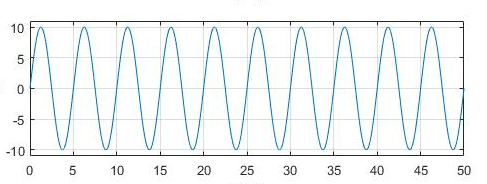
\includegraphics[height=29mm, width=45mm]{Graphics/FourierOnda.png}
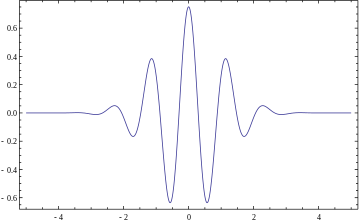
\includegraphics[scale=.33]{Graphics/FuncionWavelet.png}
\caption{Izquierda: Onda (Fourier). Derecha: Ondita (Wavelet).}
\label{wav-fourier}
\end{figure}

\begin{definition}
De manera formal, una wavelet es una funci\'on $\Psi(t)\in L^2(\mathbb{R})$ tal que la familia de funciones:
\begin{eqnarray}
\Psi_{a,b}(t)&:=&\frac{1}{\sqrt{a}}\Psi\left(\frac{t-b}{a}\right),\nonumber
\end{eqnarray}
donde $a$ y $b$ son reales que indican la escala y el desplazamiento, respectivamente, es una base ortonormal en el espacio de Hilbert $L^2(\mathbb{R})$.
\label{wav-continua}
\end{definition}

\par Este conjunto de funciones est\'an definidas en todo $\mathbb{R}$, por lo que representan funciones continuas, para los intervalos en los cuales se definen. Aunque esta forma de expresar las definici\'on de funciones wavelets es muy \'util para el an\'alisis, fundamentalmente te\'orico, de se\~nales en investigaciones cient\'ificas, puede presentar un problema para la codificaci\'on de las mismas en campos como la ingenier\'ia y las ciencias computacionales. Por ello, se define el espacio $\ell^2\left(\mathbb{Z}_N\right)=\{z(i)|0\leq i \leq N-1\}$ donde $z$ representa un vector de dimensi\'on $N$, en el cual se brindar\'a una definici\'on discreta, m\'as tratable para equipos de c\'omputo y ser\'a la que se utilizar\'a en lo adelante.\\

\begin{definition}
Se define la funci\'on wavelet discreta $\Psi(t)\in \ell^2(\mathbb{Z}_N)$ tal que la familia de funciones:
\begin{eqnarray}
\Psi_{j,k}(t)&:=&2^{\frac{j}{2}}\Psi(2^jt-k),\nonumber
\end{eqnarray}
con $j$ y $k$ enteros, es una base ortonormal en el espacio $\ell^2(\mathbb{Z}_N)$.
\label{wav-discreta}
\end{definition}

\par Como se puede apreciar, la definici\'on de wavelet discreta se obtiene al discretizar los parámetros de desplazamiento y escalamiento dentro de la definici\'on de wavelet continua:
\begin{eqnarray}
a&=&2^{-j}\nonumber\\
b&=&k2^{-j}\qquad\mbox{con $j,k\in \mathbb{Z}$}.\nonumber
\end{eqnarray}

\par A la funci\'on $\Psi$ se le llama entonces wavelet madre. En su forma discreta, cada elemento de la base wavelet constituye un vector de dimensi\'on $N$. Se ver\'a entonces c\'omo es posible obtener esta base y, por tanto, wavelet madre. A continuaci\'on se presentan un conjunto de definiciones a fin de proporcionar una notaci\'on y un algoritmo para obtener dichas wavelets.\\

\begin{definition}
Se define la transformada discreta de Fourier del vector $w\in \ell^2\left(\mathbb{Z}_N\right)$ como:
\begin{eqnarray}
\hat{w}(m)=\sum_{n=0}^{N-1}w(n)e^{\frac{-2\pi imn}{N}},\quad\forall\,m\nonumber
\end{eqnarray}
\end{definition}

\begin{definition}
Se define la reflexi\'on conjugada $\tilde{w}$ de un vector $w\in \ell^2\left(\mathbb{Z}_N\right)$ como:
\begin{eqnarray}
\tilde{w}(n)=\overline{w(-n)}=\overline{w(N-n)}.\nonumber
\end{eqnarray}
\end{definition}

\begin{definition}
Se define la convoluci\'on $\ast$ entre dos vectores $w,z\in \ell^2(\mathbb{Z}_N)$ como:
\begin{eqnarray}
(z \ast w )(n) = \sum_{i=0}^{N-1}w(i)z(n-i).\nonumber
\end{eqnarray}
\end{definition}

\begin{definition}
Sea $w\in \ell^2(\mathbb{Z}_N)$ un vector y $k\in\mathbb{Z}$, se define $R_kw$ como la traslaci\'on de $w$ por $k$ dada por:
\begin{eqnarray}
R_kw(n)=w(n-k).\nonumber
\end{eqnarray}
\end{definition}

\subsection{Banco de Filtros}

\begin{definition}
Sea $N$ divisible por $2^p$. Se define un banco de filtros wavelet de $p$ escalas a partir de dos sucesiones de vectores $u_1$, $u_2$, ..., $u_p$ y $v_1$, $v_2$, ..., $v_p$, tales que:
\begin{eqnarray}
u_j, v_j \in \ell^2 \left(\mathbb{Z}_{\frac{N}{2^{j-1}}}\right),~\forall\,j=1,2,\cdots,p,\nonumber
\end{eqnarray}
y tales que la matriz del sistema:
\begin{eqnarray}
A_j(m) = \frac{1}{\sqrt{2}}\left[\begin{array}{cc}
\hat{u}_j(m)&\hat{v}_j(m)\\
\hat{u}_j\left(m+\frac{N}{2^j}\right)&\hat{v}_j\left(m+\frac{N}{2^j}\right)
\end{array}\right],\nonumber
\end{eqnarray}
es unitaria $\forall\,m=0,1,\cdots,\frac{N}{2^j}-1,\,j=1,2,\cdots,p$.
\label{banco-filtro}
\end{definition}

\par Consid\'erese esta \'ultima definici\'on. Sea $u_j\in \ell^2\left(\mathbb{Z}_{\frac{N}{2^{j-1}}}\right)$ un vector tal que $\{R_{2k}u_j\}_{k=0}^{\frac{N}{2^j}-1}$ constituye una base ortonormal. Si se define $v_j\in \ell^2\left(\mathbb{Z}_{\frac{N}{2^{j-1}}}\right)$ tal que:
\begin{eqnarray}
v_j(n)=(-1)^{n-1}\overline{u_j(1-n)},\nonumber
\end{eqnarray}
entonces, se cumple que $\{R_{2k}u_j\}_{k=0}^{\frac{N}{2^j}-1} \cup \{R_{2k}v_j\}_{k=0}^{\frac{N}{2^j}-1}$ es una base wavelet en $\ell^2\left(\mathbb{Z}_{\frac{N}{2^{j-1}}}\right)$ y, por tanto, la matriz del sistema $A_j(m)$ es unitaria para toda $m=0,1,\cdots,\frac{N}{2^j}-1$ (ver demostraci\'on en [\textcolor{cyan}{\cite{8}}]).\\

\begin{definition}
Suponga que $N$ es divisible por $2^p$. Se define $D^p:\ell^2\left(\mathbb{Z}_N\right)\rightarrow \ell^2\left(\mathbb{Z}_{\frac{N}{2^p}}\right)$ para $z\in \ell^2\left(\mathbb{Z}_N\right)$ como:
\begin{eqnarray}
D^p(z)(n)=z(2^pn),\qquad\mbox{para $n=0,1,\cdots,M-1$.}\nonumber
\end{eqnarray}
Al operador $D$ se le denomina operador de submuestreo.
\end{definition}

\begin{definition}
Suponga que $N$ es divisible por $2^p$. Se define $U^p: \ell^2\left(\mathbb{Z}_{\frac{N}{2^p}}\right)\rightarrow \ell^2\left(\mathbb{Z}_N\right)$ para $z\in \ell^2\left(\mathbb{Z}_{\frac{N}{2^p}}\right)$ como:
\begin{eqnarray}
U^p(z)(n)=\left\{\begin{array}{ll}
z\left(\frac{n}{2^p}\right)&\quad\mbox{si $n$ es divisible por $2^p$}\\
0&\quad\mbox{en otro caso.}
\end{array}\right.\nonumber
\end{eqnarray}
Al operador $U$ se le denomina operador de sobremuestreo.
\end{definition}

\begin{definition}
Suponga que $N$ es divisible por $2^p$. Sean $u_j,v_j\in \ell^2\left(\mathbb{Z}_{\frac{N}{2^{j-1}}}\right)$. Se definen $f_j,g_j\in \ell^2\left(\mathbb{Z}_N\right)$ como:
\begin{eqnarray}
f_j&=&g_{j-1}\ast U^{j-1}(v_j),\nonumber\\
g_j&=&g_{j-1}\ast U^{j-1}(u_j),\nonumber
\end{eqnarray}
para toda $j=2,3,\cdots,p$, donde $f_1=v_1$ y $g_1=u_1$.
\end{definition}

\par Consid\'erese ahora que los vectores $u_j$ y $v_j$ de la definici\'on anterior son tomados de tal forma que la matriz del sistema $A_j(n)$ es unitaria para toda $n=0,1,\cdots,\frac{N}{2^j}-1$. Entonces, se cumple que:
\begin{eqnarray}
\{R_{2^jk}f_j\}_{k=0}^{\frac{N}{2^j}-1}\cup\{R_{2^jk}g_j\}_{k=0}^{\frac{N}{2^j}-1},\nonumber
\end{eqnarray}
constituye una base ortonormal con $\frac{N}{2^{j-1}}$ elementos (ver demostraci\'on en [\textcolor{cyan}{\cite{8}}]).

\par Como consecuencia del resultado anterior, si se desarrolla el t\'ermino $g_{j-1}$ en cada nueva ecuaci\'on se obtiene la siguiente base de $\ell^2\left(\mathbb{Z}_N\right)$:
\begin{eqnarray}
\{R_{2k}f_1\}_{k=0}^{\frac{N}{2}-1}\cup\{R_{4k}f_2\}_{k=0}^{\frac{N}{4}-1}\cup ...\cup\{R_{2^{p}k}f_{p}\}_{k=0}^{\frac{N}{2^{p}}-1}\cup\{R_{2^{p}k}g_{p}\}_{k=0}^{\frac{N}{2^{p}}-1}.\nonumber
\end{eqnarray}

\par A partir de la definici\'on~\ref{wav-discreta}, se cumple que, si se toman $\Psi_{j,k}=R_{2^jk}f_j$ y\linebreak $\Phi_{j,k}=R_{2^jk}g_j$, entonces $f_1$ y $g_1$ constituyen la wavelet madre y la wavelet padre, respectivamente.\\

\par Durante el proceso de an\'alisis de una se\~nal se aplica la llamada Transformada Wavelet Discreta que consiste en determinar los coeficientes wavelets de la se\~nal respecto a la base representada por el banco de filtros. Estos coeficientes coinciden con los valores de $z\ast\tilde{v}$ y $z\ast\tilde{u}$, m\'as a\'un, se cumple que:
\begin{eqnarray}
v\ast U(D(z\ast\tilde{v}))+u\ast U(D(z\ast\tilde{u}))=z,\nonumber
\end{eqnarray}
representa todo el proceso de an\'alisis y s\'intesis de una se\~nal $z$ usando el banco de filtros obtenido a partir de $u$ y $v$.\\

\par Como se ha podido apreciar hasta el momento, encontrar una wavelet en $\ell^2\left(\mathbb{Z}_N\right)$ se reduce a encontrar un banco de filtros en $\ell^2\left(\mathbb{Z}_N\right)$. As\'i, por ejemplo, si se toman:
\begin{eqnarray}
u&=&\left(\frac{1}{\sqrt{2}},\,\frac{1}{\sqrt{2}},0,...,0\right),\nonumber\\
v&=&\left(\frac{1}{\sqrt{2}},\,-\frac{1}{\sqrt{2}},0,...,0\right),\nonumber
\end{eqnarray}
se cumple que $\{R_{2k}v\}_{k=0}^{\frac{N}{2}-1}\cup\{R_{2k}u\}_{k=0}^{\frac{N}{2}-1}$ es una base ortonormal en $\ell^2\left(\mathbb{Z}_N\right)$ y, por tanto, la matriz del sistema es unitaria, luego es posible afirmar que se obtiene un banco de filtros a partir de $u$ y $v$. La wavelet que se obtiene a partir de este, es conocida como wavelet de Haar.\\

\par Hasta el momento se ha explicado qu\'e son las wavelets, se conocen las ventajas que posee en el an\'alisis de se\~nales respecto a las series de Fourier y que cada wavelet se reduce a encontrar un banco de filtros. Ahora el an\'alisis se enfocar\'a en este \'ultimo aspecto; la diferencia que existe entre las wavelets est\'a dada por los valores de los vectores $u$ y $v$ que son denominados, generalmente, como filtro de reconstrucci\'on de paso bajo y filtro de reconstrucci\'on de paso alto, respectivamente. Los valores de estos filtros son calculados en dependencia de la finalidad para la cual se haya creado la wavelet, esto quiere decir que, si se deseara crear una wavelet capaz de reconocer un patr\'on espec\'ifico en una se\~nal, ser\'ia necesario crear un banco de filtros basado en los valores de dicho patr\'on. Para ello, existen unas wavelets conocidas con el nombre de shapelets.\\

\subsection{Trasformada Shapelet Discreta}

\par En 2017, Rodrigo Capobianco Guido [\cite{10}] introduce la segunda generaci\'on de la Transformada Shapelet Discreta (Discrete Shapelet Transform, DST-II, por sus siglas en ingl\'es). Esta wavelet tiene la caracter\'istica de que, a diferencia de otras wavelets conocidas, fusiona tres tipos de informaci\'on: tiempo, frecuencia y forma. Se propone un procedimiento mediante el cual es posible obtener los vectores $u$ y $v$ del banco de filtros con un enfoque m\'as simple al de su predecesor, la DST-I o simplemente DST [\cite{11}].

\par El algoritmo propuesto para determinar el banco de filtros de la shapelet tiene gran similitud al usado para determinar los filtros de la wavelet de Daubechies. Por ello, se muestra en una primera instancia el algoritmo para encontrarlos en caso de esta \'ultima.

\par El c\'alculo de un banco de filtros puede ser reducido a la determinaci\'on de un \'unico vector $v$ conocido como filtro de paso alto. A partir del cual, de cumplir con las condiciones consideradas en la definici\'on~\ref{banco-filtro}, es posible determinar el valor del filtro de paso bajo $u$ y, por tanto, el banco de filtros.

\par La primera condici\'on que debe cumplir el vector $v$ en la wavelet de Daubechies es la condici\'on de energ\'ia unitaria, es decir:

\begin{eqnarray}
\sum_{k=0}^{N-1}v(k)^2=1.
\label{energiaunitaria}
\end{eqnarray}

\par La ecuaci\'on anterior est\'a muy relacionada a la segunda condici\'on que es la condici\'on de ortogonalidad, pues constituye a la vez la primera ecuaci\'on de este conjunto de igualdades. Se dan entonces $\frac{N}{2}-1$ ecuaciones relacionadas a las condiciones de ortogonalidad del filtro:

\begin{eqnarray}
\sum_{k=0}^{N-2l-1}v(k)v(k+2l)=0,\qquad\forall\,l=1,2,\cdots,\frac{N}{2}-1.
\label{ortogonalidad}
\end{eqnarray}

\par Como tercera y \'ultima condici\'on, se le imponen $\frac{N}{2}$ ecuaciones de momento de desvanecimiento, tambi\'en llamados momentos nulos:

\begin{eqnarray}
\sum_{k=0}^{N-1}v(k)k^b=0,\qquad\forall\,b=0,1,\cdots,\frac{N}{2}-1.
\label{momento-nulo}
\end{eqnarray}

\par Como se puede apreciar, la suma total de las ecuaciones es $N$, donde $N$ debe ser un n\'umero par, que coincide con el n\'umero de variables (componentes del vector $v$). Por lo tanto, se obtiene un sistema al menos compatible determinado y, en el peor caso, compatible con un n\'umero infinito de vectores posibles como candidatos al banco de filtro.

\par Una vez obtenido el valor de $v$, aplicando algunos de los m\'etodos de resoluci\'on de sistemas de ecuaciones conocidos, se determina el vector $u$, a partir de la consideraci\'on dada en la definici\'on 1.6. Se sabe que es posible tomar $v$ a partir de $u$ para que $\{R_{2k}u\}_{k=0}^{\frac{N}{2}-1} \cup \{R_{2k}v\}_{k=0}^{\frac{N}{2}-1}$ constituya una base ortonormal de $\ell^2(\mathbb{Z}_N)$ de la siguiente forma:
\begin{eqnarray}
v(n)=(-1)^{n-1}\overline{u(1-n)},\nonumber
\end{eqnarray}
sea entonces $m=1-n$, se tiene:
\begin{eqnarray}
v(1-m)&=&(-1)^{-m}\overline{u(m)},\nonumber\\
(-1)^{m}v(1-m)&=&\overline{u(m)},\nonumber\\
(-1)^{m}\overline{v(1-m)}&=&u(m).\nonumber
\end{eqnarray}

\par A partir de los vectores $u$ y $v$, se tiene el banco de filtros y, a su vez, la wavelet correspondiente. La Figura~\ref{coef-daubechies} muestra una tabla con los posibles valores de $u$ en el caso de la wavelet de Daubechies para diferentes valores de $N$.

\begin{figure}[h]
\center
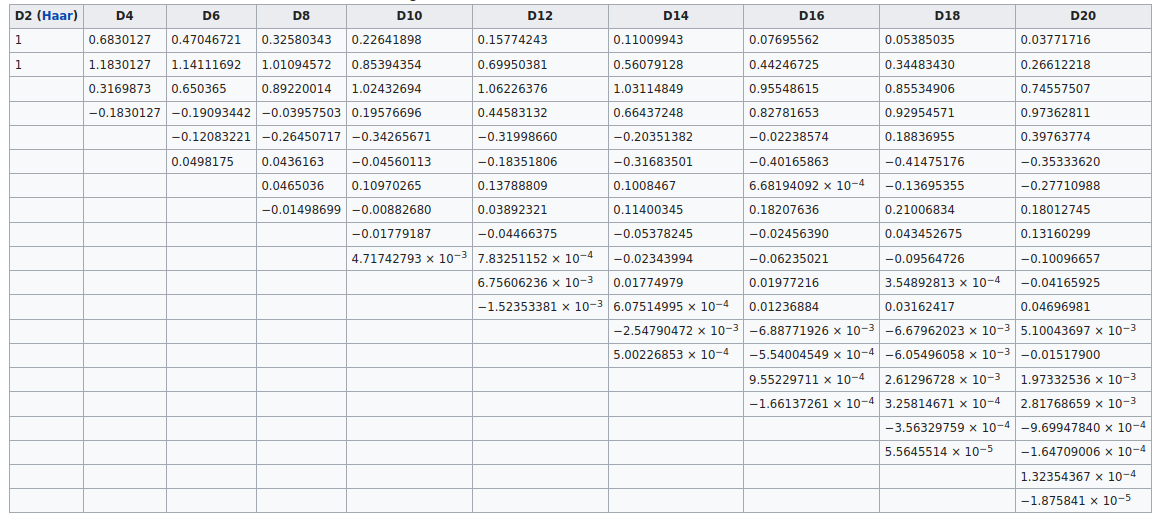
\includegraphics[scale=.35]{Graphics/Daubechies.png}
\caption{Coeficientes ortogonales de Daubechies.}
\label{coef-daubechies}
\end{figure}

\par Como se puede apreciar, las wavelets de Daubechies obtenidas ser\'an las mismas para un valor de $N$ dado y no se modificar\'an, independientemente de la se\~nal que se est\'e analizando. Si se desea realizar la tarea de detectar un patr\'on en una se\~nal no ser\'ia factible utilizar los mismos valores para cada muestra. Por ello, a la hora de construir una shapelet es necesario tener en cuenta la ``forma'' del patr\'on.

\par Las primeras dos condiciones correspondientes a la propiedad de ortogonalidad que deben cumplir los filtros (ecuaciones 1.1 y ~\ref{ortogonalidad}) son v\'alidas tambi\'en para las shapelets, pues son condiciones necesarias para que un conjunto de vectores sea considerado un banco de filtros.

\par En el caso de la tercera condici\'on, en vez de tener $\frac{N}{2}$ ecuaciones, se tomar\'an $\frac{N}{2}-2$ ecuaciones de momentos nulos. La raz\'on se debe a una cuarta condici\'on que requieren las shapelets. Supongase que se desea detectar un patr\'on $m$ y la informaci\'on que se conoce del mismo es que $m(k)=m_k$ para toda $k=0,1,\cdots,N$, las siguientes dos ecuaciones se conocen como ecuaciones de detecci\'on:
\begin{eqnarray}
\sum_{k=0}^{N}v(k)m(k)=0,
\label{matching1}\\
\sum_{k=0}^{N}v(k)m(k+1)=0.
\label{matching2}
\end{eqnarray}

\par A diferencia de las ecuaciones usadas en la DST-I, aqu\'i se consideran dos ecuaciones de detecci\'on debido a las traslaciones di\'adicas que sufre el filtro en la fase de an\'alisis de la se\~nal, que de usar una sola, podr\'ia provocar que no se detecte el patr\'on.\\

\par A continuaci\'on se muestra un ejemplo del m\'etodo propuesto. Se desea detectar el patr\'on de la Figura~\ref{patron-unidimensional} en una se\~nal de muestra, para ello es necesario determinar el banco de filtros de la shapelet correspondiente al patr\'on en cuesti\'on. Tomando $N=8$ se obtiene el siguiente sistema de ecuaciones no lineales:
\begin{eqnarray}
v(0)^2+v(1)^2+v(2)^2+v(3)^2+v(4)^2+v(5)^2+v(6)^2+v(7)^2=1,\nonumber
\end{eqnarray}
como condiciones de ortogonalidad las tres ecuaciones:
\begin{eqnarray}
v(0)v(2)+v(1)v(3)+v(2)v(4)+v(3)v(5)+v(4)v(6)+v(5)v(7)&=&0,\nonumber\\
v(0)v(4)+v(1)v(5)+v(2)v(6)+v(3)v(7)&=&0,\nonumber\\
v(0)v(6)+v(1)v(7)&=&0,\nonumber
\end{eqnarray}
dos ecuaciones de momentos nulos:
\begin{eqnarray}
v(0)+v(1)+v(2)+v(3)+v(4)+v(5)+v(6)+v(7)=0,\nonumber\\
v(1)+2v(2)+3v(3)+4v(4)+5v(5)+6v(6)+7v(7)=0,\nonumber
\end{eqnarray}
y dos ecuaciones de detecci\'on:
\begin{small}
\begin{eqnarray}
0.2v(0)+0.5v(1)+0.45v(2)+0.85v(3)+0.8v(4)-0.75v(5)+0.25v(6)+0.2v(7)=0,\nonumber\\
0.5v(0)+0.45v(1)+0.85v(2)+0.8v(3)-0.75v(4)+0.25v(5)+0.2v(6)+0.55v(7)=0.\nonumber
\end{eqnarray}
\end{small}

\begin{figure}[h]
\center
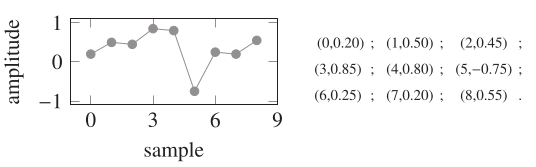
\includegraphics[scale=.5]{Graphics/Patron.png}
\caption{Ejemplo de una se\~nal patr\'on ($m$).}
\label{patron-unidimensional}
\end{figure}

\par Tras aplicar m\'etodos conocidos para la resoluci\'on de ecuaciones no lineales se obtiene como una de sus posibles soluciones:
\begin{eqnarray}
v = (-0.0834,0.1505,0.5719,-0.7055,-0.0091,-0.2784,0.2277,0.1263).\nonumber
\end{eqnarray}

\par Una vez obtenido $v$ es posible calcular el valor del resto de los filtros $u$, $\tilde{v}$ y $\tilde{u}$ que corresponden a los filtros de reconstrucci\'on pasa bajo, de an\'alisis pasa alto y an\'alisis pasa bajo respectivamente, de donde:

\begin{eqnarray}
u&=&(-0.1263,0.2277,0.2784,-0.0091,0.7055,0.5719,-0.1505,-0.0834),\nonumber\\
\tilde{v}&=&(-0.0834,0.1263,0.2277,-0.2784,-0.0091,-0.7055,0.5719,0.1505),\nonumber\\
\tilde{u}&=&(0.1505,-0.5719,-0.7055,0.0091,-0.2784,-0.2277,0.1263,0.0834).\nonumber
\end{eqnarray}

\par Al aplicar la transformada shapelet usando los filtros anteriores, se obtienen dos nuevos vectores $cA$ y $cD$ en la fase de an\'alisis que constituyen los coeficientes wavelets de la representaci\'on de la se\~nal original en la base $\{R_{2k}u\}_{k=0}^{\frac{N}{2}-1} \cup \{R_{2k}v\}_{k=0}^{\frac{N}{2}-1}$
\begin{eqnarray}
\left.\begin{array}{r}
D(z\ast\tilde{v})=cA\\
D(z\ast\tilde{u})=cD
\end{array}\right\}\mbox{fase de an\'alisis,}\nonumber
\end{eqnarray}
mientras que:
\begin{eqnarray}
\left.v\ast U(cA)+u\ast U(cD)=z\right\}\mbox{fase de s\'intesis.}\nonumber
\end{eqnarray}

\par El nuevo vector $cD$ es conocido en una dimensi\'on como el vector de detalles y es donde se almacenar\'an los valores que se necesitan para determinar la presencia o no del patr\'on que describen $u$ y $v$ dentro de la se\~nal. Para ello, se define una funci\'on de medida de similaridad $\mathbb{S}$ tal que $\mathbb{S}=e^{-\left|\mbox{\small{DST-II}}(z)\right|^{\alpha}}$, esta funci\'on enfatiza la presencia de ceros en el vector $\mbox{DST-II}(z)$ para un $0<\alpha<1$.

\par Sea la se\~nal de muestra de la Figura~\ref{signal-1d}, definida para toda $k\in \mathbb{Z}$ tal que $0\leq k \leq 63$:
\begin{eqnarray}
z(k)&=&\left\{\begin{array}{ll}
cos\left(\frac{27\pi k}{8}\right)sen\left(\frac{75\pi k}{8}\right),&\quad\mbox{para $0\leq k \leq 40$}\\
m(k),&\quad\mbox{para $41 \leq k \leq 49$}\\
cos\left(\frac{295\pi k}{32}\right)sen\left(\frac{105\pi k}{32}\right),&\quad\mbox{para $50 \leq k \leq 63$}
\end{array}\right.\nonumber
\end{eqnarray}

\begin{figure}[h]
\center
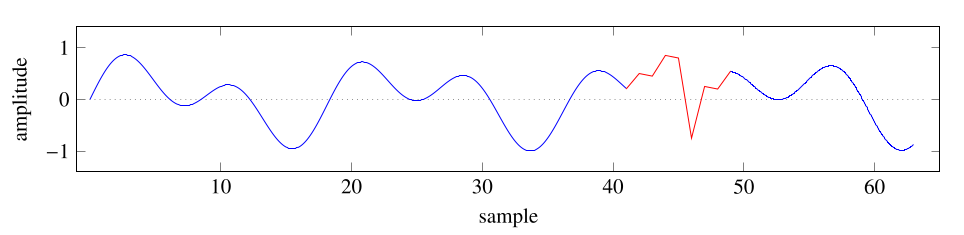
\includegraphics[scale=.4]{Graphics/Signal.png}
\caption{Se\~nal de muestra con el patr\'on $m$ incluido.}
\label{signal-1d}
\end{figure}

\par Sean $cA$ y $cD$ los vectores de aproximaci\'on y detalles, respectivamente obtenidos a partir de la DST-II. La figura~\ref{similaridad-1d} muestra los valores de estos vectores (naranja) y los valores de la medida de similaridad (azul, con $\alpha=0.1$) aplicada a cada uno de los valores de los vectores $cA$ y $cD$. Como se puede apreciar, para $k=53$ se obtiene un valor significativamente cercano a $1$ en el gr\'afico de similaridad, si se tiene en cuenta que, este valor corresponde al \'indice $k=21$ en el vector de aproximaci\'on $cD$ y, por tanto, a la posici\'on $k=42$ en la se\~nal original, entonces se puede afirmar que el algoritmo detect\'o satisfactoriamente al patr\'on $m$ en la se\~nal de muestra.

\begin{figure}[h]
\center
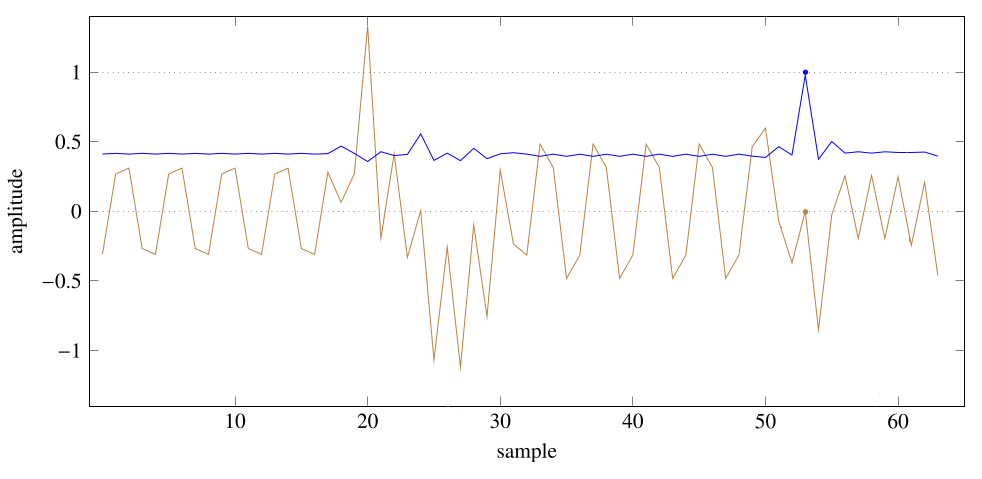
\includegraphics[scale=.4]{Graphics/Similarity.png}
\caption{Representaci\'on de los vectores de aproximaci\'on (los primeros 32 valores) y detalle (los valores entre 32 y 63) y, la medida de similaridad con el patr\'on.}
\label{similaridad-1d}
\end{figure}

\par Como parte del experimento, la medida $\mathbb{S}$ fue aplicada a los resultados obtenidos para los vectores $cA$ y $cD$ tras aplicar la transformada wavelet usando las wavelets: Haar, Daubechies 4, 6, 8, 10, 20, 30, 40, 50, 60 y 70, Symmlet 8 y 16, Coiflets 6, 12, 24, y 30, Beylkin 18 y, por \'ultimo, Vaidyanathan 24. Sin embargo DST-II fue la \'unica capaz de identificar al patr\'on $m$ dentro de la se\~nal $z$.

\section{Wavelets en dos dimensiones}\label{cap:w2d}

\par Hasta el momento se dispone de un m\'etodo para identificar un patr\'on dado en una se\~nal de muestra aplicando la transformada shapelet. Dicho m\'etodo funciona de manera efectiva en se\~nales unidimensionales, ?`que pasar\'ia entonces si se agrega una dimensi\'on m\'as? Para poder extender el concepto shapelet a dos dimensiones es necesario adaptar el conjunto de herramientas del cual se dispone en una dimensi\'on a dos dimensiones, tal que sea capaz de obtener similares resultados ya no solo para se\~nales sino tambi\'en para im\'agenes.\\

\par Anteriormente, se dieron un conjunto de definiciones para mostrar un algoritmo que permitiera, a partir de un vector, construir un banco de filtros y, por consiguiente, una base wavelet. Una imagen puede ser representada por un vector en $\ell^2(\mathbb{Z}_{N_1}\times\mathbb{Z}_{N_2})$, donde $\ell^2(\mathbb{Z}_{N_1}\times\mathbb{Z}_{N_2})=\{z(i,j)|0\leq i \leq N_1-1,\,0\leq j\leq N_2-1\}$, consid\'erese entonces dicho espacio como el punto de partida.

\subsection{Definiciones}

\par Las siguientes definiciones fueron extra\'idas de [\textcolor{cyan}{\cite{12}}].\\

\begin{definition}
Para $z\in \ell^2(\mathbb{Z}_{N_1}\times\mathbb{Z}_{N_2})$ se define $\hat{z}$ como la transformada discreta de Fourier de $z$ tal que:
\begin{eqnarray}
\hat{z}(m_1,m_2)&=&\sum_{n_1=0}^{N_1-1}\sum_{n_2=0}^{N_2-1}z(n_1,n_2)e^{\frac{-2\pi im_1n_1}{N_1}}e^{\frac{-2\pi im_2n_2}{N_2}},\qquad\forall\,m_1,m_2.\nonumber
\end{eqnarray}
\end{definition}

\begin{definition}
Para $z\in \ell^2(\mathbb{Z}_{N_1}\times\mathbb{Z}_{N_2})$ se define $\tilde{z}$ como la reflexi\'on conjugada de $z$ tal que:
\begin{eqnarray}
\tilde{z}(m_1,m_2)&=&\overline{z(-m_1,-m_2)}=\overline{z(N_1-m_1,N_2-m_2)},\qquad\forall\,m_1,m_2.\nonumber
\end{eqnarray}
\end{definition}

\begin{definition}
Para todo $w,z\in \ell^2(\mathbb{Z}_{N_1}\times\mathbb{Z}_{N_2})$ se define la convoluci\'on entre ellos como $z\ast w$ tal que:
\begin{eqnarray}
(z\ast w)(m_1,m_2)&=&\sum_{n_1=0}^{N_1-1}\sum_{n_2=0}^{N_2-1}z(m_1-n_1,m_2-n_2)w(n_1,n_2),\qquad\forall\,m_1,m_2.\nonumber
\end{eqnarray}
\end{definition}

\begin{definition}
Para $z\in \ell^2(\mathbb{Z}_{N_1}\times\mathbb{Z}_{N_2})$ y $k_1,k_2\in\mathbb{Z}$ se define $R_{k_1,k_2}{z}$ como la traslaci\'on de $z$ por $k_1,k_2$ dado por:
\begin{eqnarray}
R_{k_1,k_2}{z}(m_1,m_2)&=&z(m_1-k_1,m_2-k_2),\qquad\forall\,m_1,m_2.\nonumber
\end{eqnarray}
\end{definition}

\subsection{Banco de filtros}

\begin{theorem}
(Ver demostraci\'on en [\textcolor{cyan}{\cite{12}}]) Sup\'ongase que $M_1,M_2\in\mathbb{N}$, $N_1=2M_1$, $N_2=2M_2$ y $u_1,u_2\in \ell^2(\mathbb{Z}_{N_1}\times\mathbb{Z}_{N_2})$. Entonces, para todo $0\leq k_1 \leq M_1-1$ y\linebreak $0\leq k_2 \leq M_2-1$, $\{R_{2k_1,2k_2}u_1\}$ y $\{R_{2k_1,2k_2}u_2\}$ son conjuntos biortonormales si y solo si:
\begin{eqnarray}
u^1+u^2+u^3+u^4&=&4,\nonumber
\end{eqnarray}
donde
\begin{eqnarray}
u^1&=&\hat{u_1}(n_1,n_2)\overline{\hat{u_2}(n_1,n_2)},\nonumber\\
u^2&=&\hat{u_1}(n_1+M_1,n_2)\overline{\hat{u_2}(n_1+M_1,n_2)},\nonumber\\
u^3&=&\hat{u_1}(n_1,n_2+M_2)\overline{\hat{u_2}(n_1,n_2+M_2)},\nonumber\\
u^4&=&\hat{u_1}(n_1+M_1,n_2+M_2)\overline{\hat{u_2}(n_1+M_1,n_2+M_2)}.\nonumber
\end{eqnarray}
\end{theorem}

\begin{theorem}
(Ver demostraci\'on en [\textcolor{cyan}{\cite{12}}]) Sup\'ongase que $M_1,M_2\in\mathbb{N}$, $N_1=2M_1$, $N_2=2M_2$ y $u_i,v_i\in \ell^2(\mathbb{Z}_{N_1}\times\mathbb{Z}_{N_2})$, para toda $i=0,1,2,3$. Entonces, para todo\linebreak $0\leq k_1 \leq M_1-1$ y $0\leq k_2 \leq M_2-1$,
\begin{eqnarray}
\bigcup_{m=0}^{3}\{R_{2k_1,2k_2}u_m\}\mbox{ y }\bigcup_{m=0}^{3}\{R_{2k_1,2k_2}v_m\},\nonumber
\end{eqnarray}
son conjuntos biortogonales de $\ell^2(\mathbb{Z}_{N_1}\times\mathbb{Z}_{N_2})$ si y solo si:
\begin{eqnarray}
A_u(n_1,n_2)^T\overline{A_v(n_1,n_2)}=\left[\begin{array}{cccc}
1&0&0&0\\0&1&0&0\\0&0&1&0\\0&0&0&1
\end{array}\right],\nonumber
\end{eqnarray}
para todo $0\leq n_1 \leq M_1-1$, $0\leq n_2 \leq M_2-1$, donde $A_u(n_1,n_2)$ es la matriz cuya $m-$\'esima columna ($m=0,1,2,3$) es:
\begin{eqnarray}
\frac{1}{2}\left[\begin{array}{c}
\hat{u}_m(n_1,n_2)\\
\hat{u}_m(n_1+M_1,n_2)\\
\hat{u}_m(n_1,n_2+M_2)\\
\hat{u}_m(n_1+M_1,n_2+M_2)
\end{array}\right],\nonumber
\end{eqnarray}
y $A_v(n_1,n_2)$ es la matriz cuya $m-$\'esima columna ($m=0,1,2,3$) es:
\begin{eqnarray}
\frac{1}{2}\left[\begin{array}{c}
\hat{v}_m(n_1,n_2)\\
\hat{v}_m(n_1+M_1,n_2)\\
\hat{v}_m(n_1,n_2+M_2)\\
\hat{v}_m(n_1+M_1,n_2+M_2)
\end{array}\right].\nonumber
\end{eqnarray}
\label{biortogonalidad}
\end{theorem}

\begin{definition}
Suponga que $M_1,M_2\in\mathbb{N}$, $N_1=2M_1$ y $N_2=2M_2$. Se definen los operadores $$D^l: \ell^2(\mathbb{Z}_{N_1}\times\mathbb{Z}_{N_2})\rightarrow \ell^2\left(\mathbb{Z}_{\frac{N_1}{2^l}}\times\mathbb{Z}_{\frac{N_2}{2^l}}\right),$$ de submuestreo y $$U^l: \ell^2\left(\mathbb{Z}_{\frac{N_1}{2^l}}\times\mathbb{Z}_{\frac{N_2}{2^l}}\right)\rightarrow \ell^2(\mathbb{Z}_{N_1}\times\mathbb{Z}_{N_2}),$$ de sobremuestreo como:
\begin{eqnarray}
D^l(z)(n_1,n_2)=z(2^ln_1,2^ln_2),\qquad\forall\,z\in \ell^2(\mathbb{Z}_{N_1}\times\mathbb{Z}_{N_2}),\nonumber
\end{eqnarray}
y
\begin{eqnarray}
U^l(z)(n_1,n_2)&=&\left\{\begin{array}{rr}
z\left(\frac{n_1}{2^l},\frac{n_2}{2^l}\right),&\quad 2^l | n_1,\, 2^l|n_2\\
0,&\quad\mbox{en otro caso,}
\end{array}\right.\nonumber\\
\forall\,z&\in &\ell^2\left(\mathbb{Z}_{\frac{N_1}{2^l}}\times\mathbb{Z}_{\frac{N_2}{2^l}}\right),\nonumber
\end{eqnarray}
donde $D^1=D$, $U^1=U$ y $D^l(z)=(D\circ D^{l-1})(z)$, $U^l(z)=(U\circ U^{l-1})(z)$ para $l>1$.
\end{definition}

\begin{theorem}
(Ver demostraci\'on en [\textcolor{cyan}{\cite{12}}]) Sup\'ongase que $M_1,M_2\in\mathbb{N}$, $N_1=2M_1$, $N_2=2M_2$ y $u_0,u_1,u_2,u_3,s_0,s_1,s_2,s_3\in \ell^2(\mathbb{Z}_{N_1}\times\mathbb{Z}_{N_2})$. Sea la matriz $A(n_1,n_2)$ definida como en el Teorema 1.2, entonces se tiene una reconstrucci\'on perfecta:
\begin{eqnarray}
\sum_{i=0}^3 \tilde{s}_i\ast U(D(z\ast\tilde{u}_i))=z,\nonumber
\end{eqnarray}
para toda $z\in \ell^2(\mathbb{Z}_{N_1}\times\mathbb{Z}_{N_2})$, si y solo si:
\begin{eqnarray}
A(n_1,n_2)\left[\begin{array}{c}
\hat{s}_0\\ \hat{s}_1\\ \hat{s}_2\\ \hat{s}_3
\end{array}\right]=\left[\begin{array}{c}
2\\0\\0\\0
\end{array}\right],\nonumber
\end{eqnarray}
para todo $n_1,n_2$. En el caso de que $A(n_1,n_2)$ sea unitaria, entonces $s_i=\tilde{u}_i$ para $i=0,1,2,3$.
\label{reconstruccion-perfecta}
\end{theorem}

\par De los teoremas 1.2 y 1.3 se sabe que si:
\begin{eqnarray}
\bigcup_{m=0}^{3}\{R_{2k_1,2k_2}u_m\},\nonumber
\end{eqnarray}
es un conjunto biortogonal consigo mismo en $\ell^2(\mathbb{Z}_{N_1}\times\mathbb{Z}_{N_2})$ entonces la matriz $A(n_1,n_2)$ es unitaria y, por tanto:
\begin{eqnarray}
\sum_{i=0}^3 u_i\ast U(D(z\ast\tilde{u}_i))=z,\nonumber
\end{eqnarray}
constituye una reconstrucci\'on perfecta de una imagen $z$. Esto quiere decir que al igual que en una sola dimensi\'on, el problema de crear una base wavelet que permita detectar un patr\'on, se reduce al c\'alculo efectivo de un banco de filtros $\{u_i\}\cup\{\tilde{u}_i\}$, ahora biortogonal. Este constituye el pr\'oximo paso en la tarea de crear una shapelet de dos dimensiones.\\
\chapter{Propuesta}\label{chapter:proposal}

\par Hasta el momento se conoce como crear un banco de filtros en $\ell^2(\mathbb{Z}_N)$ tal que la DST-II sea capaz de reconocer un patr\'on en una se\~nal unidimensional. Tal como se vio en la secci\'on 1.2, una im\'agen puede ser definida como un vector en $\ell^2(\mathbb{Z}_{N_1}\times\mathbb{Z}_{N_2})$ al igual que un patr\'on. Si bien, en el estudio de la transformada de Shapelet de una dimensi\'on era posible construir un filtro que reconociese un patr\'on dado, dicha tarea tambi\'en es posible realizarla en dos dimensiones, aunque para ello sea necesario realizar algunos ajustes y consideraciones extras.\\

\section{Definici\'on del filtro}

\par Como bien se sabe, para determinar el banco de filtros de la Shapelet se debe resolver primeramente un sistema no lineal cuyas variables son las componentes del vector que se usar\'a para construir la base wavelet. Dicho vector pertenece al espacio $\ell^2(\mathbb{Z}_{N_1}\times\mathbb{Z}_{N_2})$ por lo que contiene un total de $N_1N_2$ componentes. A la hora de resolver el sistema de ecuaciones se estar\'ia tratando con un sistema sumamente costoso para los equipos de c\'omputos actuales. Por tanto, es necesario encontrar una alternativa para obtener dicho vector.\\

\par Seg\'un se analiz\'o anteriormente, la resoluci\'on del sistema de ecuaciones no lineal que se obtiene tratando con vectores en una dimensi\'on es m\'as factible que la de dos dimensiones; entonces, ?`ser\'ia posible construir un vector en $\ell^2(\mathbb{Z}_{N_1}\times\mathbb{Z}_{N_2})$ a partir de un vector en $\ell^2(\mathbb{Z}_N)$?

\par Suponga que $N$ es un entro positivo par y que se tienen dos vetores $v_0,v_1\in\ell^2(\mathbb{Z}_N)$ tal que $\{R_{2k}v_0\}_{k=0}^{\frac{N}{2}-1}\cup\{R_{2k}v_1\}_{k=0}^{\frac{N}{2}-1}$ constituye una base ortonormal de $\ell^2(\mathbb{Z}_N)$ y cuatro vectores $w_{0,0},w_{0,1},w_{1,0},w_{1,1}\in\ell^2(\mathbb{Z}_N\times\mathbb{Z}_N)$ tal que:
\begin{eqnarray}
\begin{array}{c}
w_{0,0}(n_1,n_2)=v_0(n_1)v_0(n_2)\\
w_{0,1}(n_1,n_2)=v_0(n_1)v_1(n_2)\\
w_{1,0}(n_1,n_2)=v_1(n_1)v_0(n_2)\\
w_{1,1}(n_1,n_2)=v_1(n_1)v_1(n_2)
\label{definicion-filtro-2d}
\end{array}
\end{eqnarray}
para todo $w_{i,j}$ con $i,j\in\{0,1\}$ entonces se cumple que:
\begin{eqnarray}
\hat{w}_{i,j}(m_1,m_2)&=&\sum_{n_1=0}^{N-1}\sum_{n_2=0}^{N-1}w_{i,j}(n_1,n_2)e^{\frac{-2\pi im_1n_1}{N}}e^{\frac{-2\pi im_2n_2}{N}}\nonumber\\
&=&\sum_{n_1=0}^{N-1}\sum_{n_2=0}^{N-1}v_i(n_1)v_j(n_2)e^{\frac{-2\pi im_1n_1}{N}}e^{\frac{-2\pi im_2n_2}{N}}\nonumber\\
&=&\left(\sum_{n_1=0}^{N-1}v_i(n_1)e^{\frac{-2\pi im_1n_1}{N}}\right)\left(\sum_{n_2=0}^{N-1}v_j(n_2)e^{\frac{-2\pi im_2n_2}{N}}\right)\nonumber\\
\hat{w}_{i,j}(m_1,m_2)&=&\hat{v}_i(m_1)\hat{v}_j(m_2)\nonumber
\end{eqnarray}
con lo cual se tiene una expresi\'on para $\hat{w}_{i,j}$ en funci\'on de los vectores $v_i$ y $v_j$ que lo componen. Considere ahora el teorema 1.1, tal que $u^1$, $u^2$, $u^3$ y $u^4$ se definen como:
\begin{eqnarray}
u^1&=&\hat{w}_{i_1,j_1}(m_1,m_2)\overline{\hat{w}_{i_2,j_2}(m_1,m_2)}=\hat{v}_{i_1}(m_1)\hat{v}_{j_1}(m_2)\overline{\hat{v}_{i_2}(m_1)}\overline{\hat{v}_{j_2}(m_2)}\nonumber\\
u^2&=&\hat{w}_{i_1,j_1}\left(m_1,m_2+\frac{N}{2}\right)\overline{\hat{w}_{i_2,j_2}\left(m_1,m_2+\frac{N}{2}\right)}\nonumber\\&=&\hat{v}_{i_1}(m_1)\hat{v}_{j_1}\left(m_2+\frac{N}{2}\right)\overline{\hat{v}_{i_2}(m_1)}\overline{\hat{v}_{j_2}\left(m_2+\frac{N}{2}\right)}\nonumber\\
u^3&=&\hat{w}_{i_1,j_1}\left(m_1+\frac{N}{2},m_2\right)\overline{\hat{w}_{i_2,j_2}\left(m_1+\frac{N}{2},m_2\right)}\nonumber\\&=&\hat{v}_{i_1}\left(m_1+\frac{N}{2}\right)\hat{v}_{j_1}\left(m_2\right)\overline{\hat{v}_{i_2}\left(m_1+\frac{N}{2}\right)}\overline{\hat{v}_{j_2}\left(m_2\right)}\nonumber\\
u^4&=&\hat{w}_{i_1,j_1}\left(m_1+\frac{N}{2},m_2+\frac{N}{2}\right)\overline{\hat{w}_{i_2,j_2}\left(m_1+\frac{N}{2},m_2+\frac{N}{2}\right)}\nonumber\\&=&\hat{v}_{i_1}\left(m_1+\frac{N}{2}\right)\hat{v}_{j_1}\left(m_2+\frac{N}{2}\right)\overline{\hat{v}_{i_2}\left(m_1+\frac{N}{2}\right)}\overline{\hat{v}_{j_2}\left(m_2+\frac{N}{2}\right)}\nonumber
\end{eqnarray}
\par Sea $s=u^1+u^2+u^3+u^4$, hallando factor com\'un $\hat{v}_{i_1}(m_1)\overline{\hat{v}_{i_2}(m_1)}$ y\linebreak $\hat{v}_{i_1}\left(m_1+\frac{N}{2}\right)\overline{\hat{v}_{i_2}\left(m_1+\frac{N}{2}\right)}$ se tiene:
\begin{scriptsize}
\begin{eqnarray}
s=\left(\hat{v}_{i_1}(m_1)\overline{\hat{v}_{i_2}(m_1)}+\hat{v}_{i_1}\left(m_1+\frac{N}{2}\right)\overline{\hat{v}_{i_2}\left(m_1+\frac{N}{2}\right)}\right)\left(\hat{v}_{j_1}(m_2)\overline{\hat{v}_{j_2}(m_2)}+\hat{v}_{j_1}\left(m_2+\frac{N}{2}\right)\overline{\hat{v}_{j_2}\left(m_2+\frac{N}{2}\right)}\right)\nonumber
\end{eqnarray}
\end{scriptsize}
\par Como $\{R_{2k}v_0\}_{k=0}^{\frac{N}{2}-1}\cup\{R_{2k}v_1\}_{k=0}^{\frac{N}{2}-1}$ constituye una base ortonormal de $\ell^2(\mathbb{Z}_N)$, se cumple que la matriz:
\begin{eqnarray}
\frac{1}{\sqrt{2}}\left[\begin{array}{cc}
\hat{v}_0(n)&\hat{v}_1(n)\\
\hat{v}_0\left(n+\frac{N}{2}\right)&\hat{v}_1\left(n+\frac{N}{2}\right)
\end{array}\right]\nonumber
\end{eqnarray}
es unitaria para toda $n$. Esto quiere decir que:
\begin{eqnarray}
\hat{v}_i(n)\overline{\hat{v}_j(n)}+\hat{v}_i\left(n+\frac{N}{2}\right)\overline{\hat{v}_j\left(n+\frac{N}{2}\right)}=\left\{\begin{array}{ll}
2,&\quad\mbox{si $i=j$}\\
0,&\quad\mbox{si $i\neq j$}
\end{array}\right.\nonumber
\end{eqnarray}
por lo tanto:
\begin{eqnarray}
s&=&\left\{\begin{array}{ll}
4,&\quad\mbox{si $i_1=i_2$ y $j_1=j_2$}\\
0,&\quad\mbox{en caso contrario}
\end{array}\right.\nonumber
\end{eqnarray}
y el conjunto $\displaystyle\bigcup_{i,j\in\{0,1\}}\{R_{2k_1,2k_2}w_{i,j}\}_{k_1=0,k_2=0}^{\frac{N}{2}-1,\frac{N}{2}-1}$ constituye un conjunto biortogonal en $\ell^2(\mathbb{Z}_N\times\mathbb{Z}_N)$. Este \'ultimo resultado trae como implicaci\'on que:
\begin{eqnarray}
\sum_{i=0}^1\sum_{j=0}^1w_{i,j}\ast U(D(z\ast\tilde{w}_{i,j}))&=&z\nonumber
\end{eqnarray}
constituya una reconstrucci\'on perfecta de $z$. Volviendo entonces a la interrogante de si era posible construir un filtro de dos dimensiones a partir de un vector de una dimensi\'on, si se define el vector de dos dimensiones como en~\ref{definicion-filtro-2d} se obtiene el filtro deseado. La \'unica condici\'on que debe cumplir es que $N_1=N_2=N$.

\section{C\'alculo del filtro}

\par Nuestro problema se reduce entonces a determinar un conjunto de vectores $v_0,v_1\in\ell^2(\mathbb{Z}_N)$ tal que $\{R_{2k}v_0\}_{k=0}^{\frac{N}{2}-1}\cup\{R_{2k}v_1\}_{k=0}^{\frac{N}{2}-1}$ constituya una base ortonormal en dicho espacio. Sin embargo en la secci\'on 1.1.3 se brinda un algoritmo para hallar dichos vectores a partir de un patr\'on de muestra. Por tanto, nuestro problema de detectar un patr\'on en dos dimensiones se reduce al problema de detectar un patr\'on en una dimensi\'on. Analizemos nuevamente las condiciones que deben cumplirse para el c\'alculo del filtro.\\

\par La primera condici\'on que deb\'ia cumplir $v$ era la condici\'on de energ\'ia unitaria (vea ecuaci\'on 1.1), mientras que la segunda condici\'on era la de ortogonalidad (ver ecuaci\'on 1.2). La tercera y cuarta condiciones representaban el momento nulo y las ecuaciones de \textit{matching} respectivamente. Deteng\'amonos en estas \'ultimas.

\par Cuando se proponen las ecuaciones de \textit{matching} en una dimensi\'on son necesarias dos ecuaciones, esto se deb\'ia a que las traslaciones di\'adicas mantienen la paridad del \'indice inicial tomado en la se\~nal de prueba para realizar la convoluci\'on con el filtro, y si el patr\'on estuviese insertado en la se\~nal pero en una posici\'on con paridad distinta, entonces no hubiese sido posible detectarlo. Para resolver este problema se utilizan dos ecuaciones en vez de una. Para el caso de dos dimensiones se puede presentar el mismo problema, sin embargo ya no solo ocurrir\'ia al desplazar el \'indice de las columnas sino tambi\'en el de las filas, por ello ser\'ian necesario utilizar cuatro ecuaciones de \textit{matching} para el proceso de determinaci\'on del filtro.
\par Al a\~nadir dos nuevas ecuaciones de \textit{matching} el sistema se puede volver incompatible, para evitarlo se eliminan dos ecuaciones m\'as de momento nulo. De esta forma, la tercera condici\'on la constituyen $\frac{N}{2}-4$ ecuaciones de desvanecimiento:
\begin{eqnarray}
\sum_{k=0}^{N-1}v(k)k^b=0,\qquad\forall b=0,1,...,\frac{N}{2}-5\nonumber
\end{eqnarray}
mientras que la cuarta condici\'on est\'a dada por las siguientes ecuaciones de \textit{matching}:
\begin{eqnarray}
&&\sum_{n_1=0}^{N-1}\sum_{n_2=0}^{N-1}v(n_1)v(n_2)m(n_1,n_2)=0\nonumber\\
&&\sum_{n_1=0}^{N-1}\sum_{n_2=0}^{N-1}v(n_1)v(n_2)m(n_1,n_2+1)=0\nonumber\\
&&\sum_{n_1=0}^{N-1}\sum_{n_2=0}^{N-1}v(n_1)v(n_2)m(n_1+1,n_2)=0\nonumber\\
&&\sum_{n_1=0}^{N-1}\sum_{n_2=0}^{N-1}v(n_1)v(n_2)m(n_1+1,n_2+1)=0\nonumber
\end{eqnarray}
donde $m$ representa un patr\'on de $\ell^2(\mathbb{Z}_{N+1}\times\mathbb{Z}_{N+1})$.\\

\par Como se puede apreciar, para el c\'alculo del filtro es necesario resolver un sistema de ecuaciones no lineales de $N$ variables con $N$ ecuaciones al igual que en el caso de una dimensi\'on. Lo cual constituye una reducci\'on significativa del tiempo te\'orico que se ten\'ia anteriormente.\\

\par Una vez resuelto el sistema aplicando alg\'un m\'etodo de resoluci\'on de sistemas de ecuaciones, se obtienen los valores de $v$ con los cuales se construyen los filtros en dos dimensiones y se aplica la DST\_II. Para ello se realiza la fase de an\'alisis de la imagen, obteniendose 4 nuevas im\'agenes $cA$, $cH$, $cV$ y $cD$ llamadas im\'agen de aproximaci\'on (obtenida con $D(z\ast w_{1,1})$), matriz de detalles horizontales (obtenida con $D(z\ast w_{0,1})$), matriz de detalles verticales (obtenida con $D(z\ast w_{1,0})$) y matriz de detalles (obtenida con $D(z\ast w_{0,0})$) respectivamente.

\par Al igual que en el caso de una dimensi\'on. El valor que indica la presencia del patr\'on se encuentra en la matriz de detalles $cD$ por lo que aplicando la medida de similitud propuesta en la secci\'on 1.1.3 se selecciona el \'indice m\'as cercano a $1$ como la localizaci\'on del patr\'on en la im\'agen.\\

\par Si bien hasta ahora solo se tiene una idea te\'orica del funcionamiento del algoritmo a continuaci\'on se presenta la implementaci\'on del mismo en correspondencia con resultados obtenidos durante los experimentos realizados.
\chapter{Experimentos}\label{chapter:implementation}

\par La implementaci\'on del algoritmo de reconocimiento de patrones propuesto se realiz\'o en el lenguaje de programaci\'on Python [\cite{22}]. La raz\'on principal: el conjunto de bibliotecas que incluye, tanto para la resoluci\'on del sistema de ecuaciones, como para determinar la transformada wavelet de un vector, lo mismo en $L^2(\mathbb{Z}_N)$ que en $L^2(\mathbb{Z}_{N_1}\times\mathbb{Z}_{N_2})$.

\par El programa se descompone en dos algoritmos y cada algoritmo en dos partes, es decir: un primer algoritmo para la detecci\'on de patrones unidimensionales en una se\~nal y un segundo para detectar un patr\'on de dimensiones cuadradas en una imagen o mamograf\'ia. En la primera fase de cada algoritmo, se plantea el sistema de ecuaciones cuya soluci\'on es el filtro de paso alto y se le da soluci\'on empleando el m\'etodo num\'erico que se mostrar\'a a continuaci\'on, mientras que en la segunda fase, se toma la wavelet creada a partir del banco de filtro con el vector hallado y se determina la transformada de la imagen de muestra (la cual no necesita ser cuadrada), tras la cual se obtienen las cuatro matrices o im\'agenes mencionadas anteriormente; de ellas se analiza la martiz $cD$ en busca de valores cercanos a cero con la funci\'on de similaridad $\mathbb{S}$ y se seleccionan los mejores candidatos de ocurrencia del patr\'on.\\

\par El problema principal del algoritmo es la resoluci\'on del sistema de ecuaciones no lineales. Por lo que se analizar\'a primero este punto antes de entrar en la implementaci\'on del programa en general.\\

\section{M\'etodos para resolver sistemas de ecuaciones no lineales}

\par Para la resoluci\'on del sistema no lineal, se consideraron varios m\'etodos num\'ericos tales como: Newton, Cuasi-Newton, descenso por gradiente, Runge-Kutta y otro empleado para la resoluci\'on de modelos de optimizaci\'on. Se analizar\'an cada uno de ellos y se determinar\'a cu\'al producir\'ia un resultado m\'as cercano al que se desea obtener.

\subsection{M\'etodo de Newton}

\par En el caso del m\'etodo de Newton [\cite{23}], consiste en un algoritmo iterativo, que en cada iteraci\'on actualiza el valor $x_0$ inicial y el jacobiano del sistema, a fin de que $x_0$ siempre se encuentre en una vecindad cada vez m\'as cercana de la ra\'iz del sistema. Este m\'etodo es muy efectivo en peque\~nos sistemas de ecuaciones y converge r\'apidamente en caso de que se tome un valor inicial relativamente cercano a la ra\'iz. Sin embargo, el problema anteriormente planteado no entra dentro de dichos sistemas de ecuaciones, ya que la dimensi\'on de los vectores que se usar\'an para el filtro pueden ser bastante grandes, por lo que la posibilidad de encontrar un primer valor $x_0$ cercano a la ra\'iz se hace muy peque\~na y en muchos casos el algoritmo podr\'ia no converger.\\

\par La Figura 3.1 muestra la efectividad del m\'etodo de Newton para distintas dimensiones del sistema de ecuaciones.

\begin{figure}[h]
\center
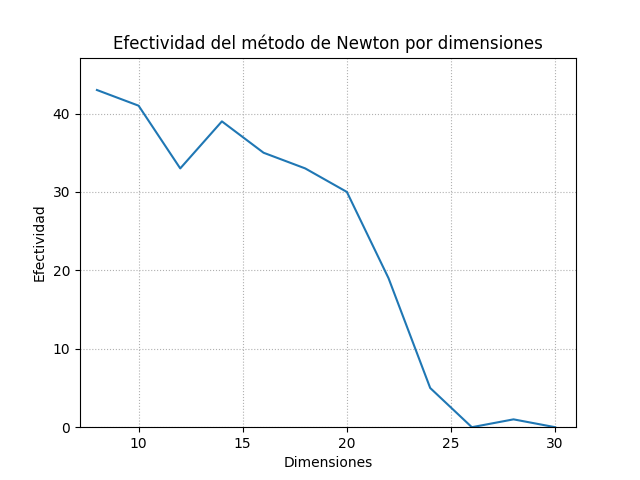
\includegraphics[scale=.45]{Graphics/Newton.png}
\caption{Efectividad (\%) del m\'etodo de Newton en el modelo para un aumento de la dimensi\'on.}
\end{figure}

\par Durante el experimento, se ejecut\'o el m\'etodo $100$ veces por cada dimensi\'on y se determin\'o el valor de la efectividad, dada el porciento que representa la cantidad de casos en los cuales el algoritmo converge satisfactoriamente, del total de casos. Como se puede apreciar, con este m\'etodo se pueden obtener valores correctos hasta con sistemas de dimensi\'on $N=26$, aunque para estos \'ultmos valores la posibilidad de encontrarlos es muy baja.

\subsection{M\'etodo Cuasi-Newton}

\par Por otro lado, el m\'etodo Cuasi-Newton [\cite{23}] constituye una mejora del m\'etodo de Newton en el sentido de que no es necesario hallar en cada iteraci\'on la inversa del jacobiano del sistema, sino que utiliza una matriz definida positiva para aproximar la inversa de la matriz hessiana, simplificando de esta forma el proceso. Sin embargo, como el m\'etodo de Newton, requiere un valor inicial $x_0$ cercano a la ra\'iz para converger.

\par Usando el mismo experimento que en el m\'etodo de Newton, se tomaron $100$ patrones aleatorios para cada dimensi\'on y se determin\'o la efectividad del m\'etodo Cuasi-Newton Broyden-Fletcher-Goldfarb-Shanno (BFGS). La Figura 3.2 muestra los resultados del an\'alisis.\\

\begin{figure}[h]
\center
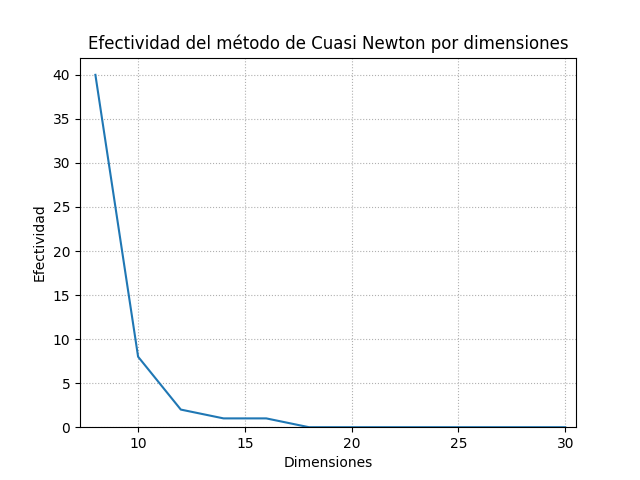
\includegraphics[scale=.4]{Graphics/CuasiNewton.png}
\caption{Efectividad (\%) del m\'etodo Cuasi-Newton en el modelo para un aumento de la dimensi\'on.}
\end{figure}

\par Como puede apreciar, inicialmente tiene una efectividad del $40\%$ para un sistema de dimensi\'on $8$, sin embargo, con un aumento de esta, comienza a reducir hasta que, a partir de $N=18$ se vuelve inefectivo.

\subsection{M\'etodo de Descenso por Gradiente}

\par El m\'etodo del descenso por gradiente [\cite{23}] es un m\'etodo usado para la determinaci\'on de m\'inimos, por lo tanto, para usar este m\'etodo fue necesario trabajar con la norma de del vector formado por las ecuaciones del sistema, de esta forma el valor $x$ que minimice la norma constituye la ra\'iz en el sistema original. La idea de optimizaci\'on de este m\'etodo, es usar la direcci\'on contraria al gradiente en el punto actual como direcci\'on de b\'usqueda, moverse una distancia $\alpha$ y volver a repetir la operaci\'on. A medida que vaya acerc\'andose al m\'inimo, la distancia $\alpha$ se reduce y m\'as lenta es la convergencia. El problema fundamental de este m\'etodo es que puede converger a m\'inimos locales, muy lejos de la ra\'iz verdadera del sistema y esto podr\'ia traer dificultades a la hora de detectar el patr\'on.\\\

\par La Figura 3.3 muestra la efectividad de este m\'etodo para $12$ valores de dimensiones distintas.\\

\begin{figure}[h]
\center
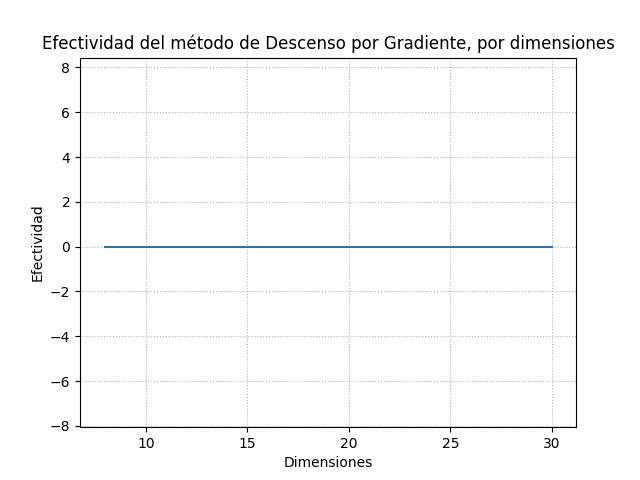
\includegraphics[scale=.45]{Graphics/DescensoGradiente.png}
\caption{Efectividad (\%) del m\'etodo de descenso por gradiente en el modelo para un aumento de la dimensi\'on.}
\end{figure}

\par Aunque al compararlo con los primeros m\'etodos vistos, r\'apidamente ser\'ia descartado, puede ser \'util como un m\'etodo de aproximaci\'on inicial.

\subsection{M\'etodo de Runge-Kutta}

\par El pr\'oximo m\'etodo es el de Runge-Kutta [\cite{23}]. Este es un m\'etodo num\'erico que, al igual que el m\'etodo de Newton, usa el jacobiano del sistema. M\'as a\'un, 
los m\'etodos de Runge Kutta son generalizaciones de la f\'ormula de Euler:
\begin{eqnarray}
x_{i+1}=x_{i}+hf(t_i,x_i),\nonumber
\end{eqnarray}
donde el valor de $f$ es reemplazado por un promedio ponderado de valores de $f$ en el intervalo $t_i\leq t \leq t_{i+1}$. Es decir,
\begin{eqnarray}
x_{i+1}=x_i+h(w_1k_1+w_2k_2+...+w_mk_m).\nonumber
\end{eqnarray}
En este caso se usar\'a Runge-Kutta de orden 4. Realizando el mismo experimento que con los m\'etodos anteriores, se obtiene el resultado mostrado en la Figura 3.4.\\

\begin{figure}[h]
\center
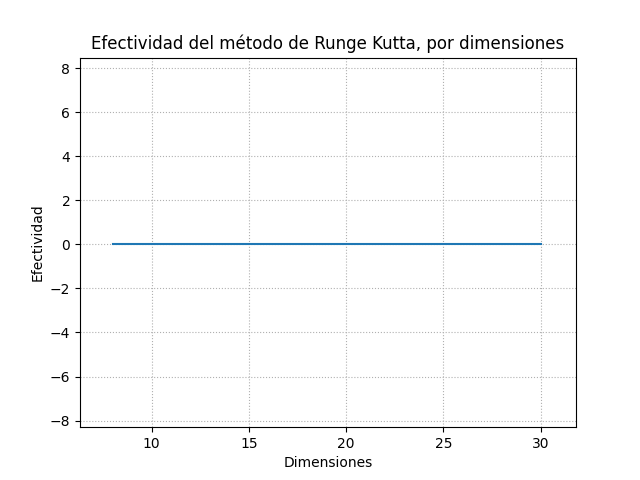
\includegraphics[scale=.4]{Graphics/RungeKutta.png}
\caption{Efectividad (\%) del m\'etodo de Runge-Kutta en el modelo para un aumento de la dimensi\'on.}
\end{figure}

\subsection{Gekko}

\par El \'ultimo m\'etodo que se analizar\'a constituye un m\'etodo usado para la resoluci\'on de problemas de maximizaci\'on y minimizaci\'on de funciones. Como parte de las bibliotecas de Python, se encuentra \textit{gekko} [\cite{13}]. \textit{Gekko} es un paquete de optimizaci\'on y aprendizaje autom\'atico que usa diferenciaci\'on autom\'atica y algoritmos basados en gradientes como APOPT (Advanced Process OPTimizer) [\cite{25}] o IPOPT (Interior Point OPTimizer) [\cite{26}] para encontrar soluci\'on a problemas de optimizaci\'on. Si cada ecuaci\'on constituye una restricci\'on y se considera la norma de las restricciones como la funci\'on objetivo, entonces es posible transformar el sistema de ecuaciones no lineales en un modelo de optimizaci\'on no lineal. Al usar \textit{gekko} para resolver los sistemas con distintas dimensiones, se obtienen los datos mostrados en la Figura 3.5.\\

\begin{figure}[h]
\center
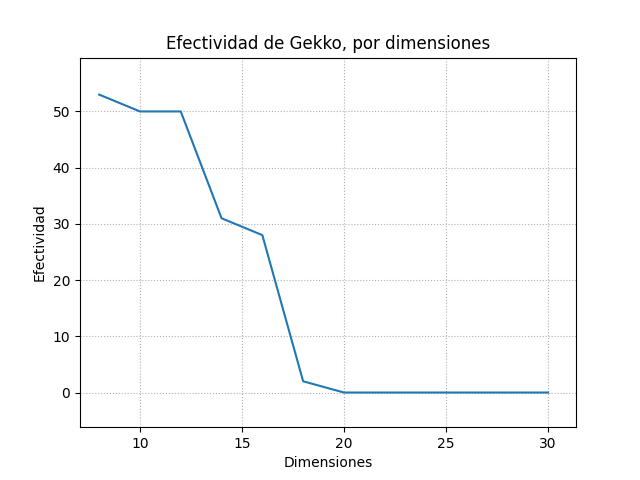
\includegraphics[scale=.4]{Graphics/Gekko.png}
\caption{Efectividad (\%) del m\'etodo de Gekko en el modelo para un aumento de la dimensi\'on.}
\end{figure}

\par En comparaci\'on con los primeros dos m\'etodos, aunque a partir de un valor de dimensi\'on dado se vuelve ineficiente, muestra un comportamiento con valores de efectividad muy buenos en comparaci\'on con el m\'etodo Cuasi-Newton pero inferiores a los de Newton.

\subsection{Mejores Resultados}

\par Hasta el momento se han analizado los m\'etodos por separado, de los cuales el m\'etodo de Newton a dado los mejores resultados. Tal como se mencion\'o varios de ellos dependen de una buena aproximaci\'on inicial. Dado que el m\'etodo del descenso por gradiente y Runge-Kutta no entran dentro de estos, se usar\'an para lograr una buena aproximaci\'on inicial y, posteriormente, aplicar alguno de los otros m\'etodos propuestos. Realizando nuevamente el experimento, usando cada m\'etodo de aproximaci\'on inicial con cada m\'etodo para encontrar la ra\'iz del sistema, se obtienen los resultados mostrados en la Figura 3.6.\\

\begin{figure}[h]
  \begin{center}
    \subfigure[\begin{scriptsize}
        Descenso por Gradiente y Newton
        \end{scriptsize}]{
        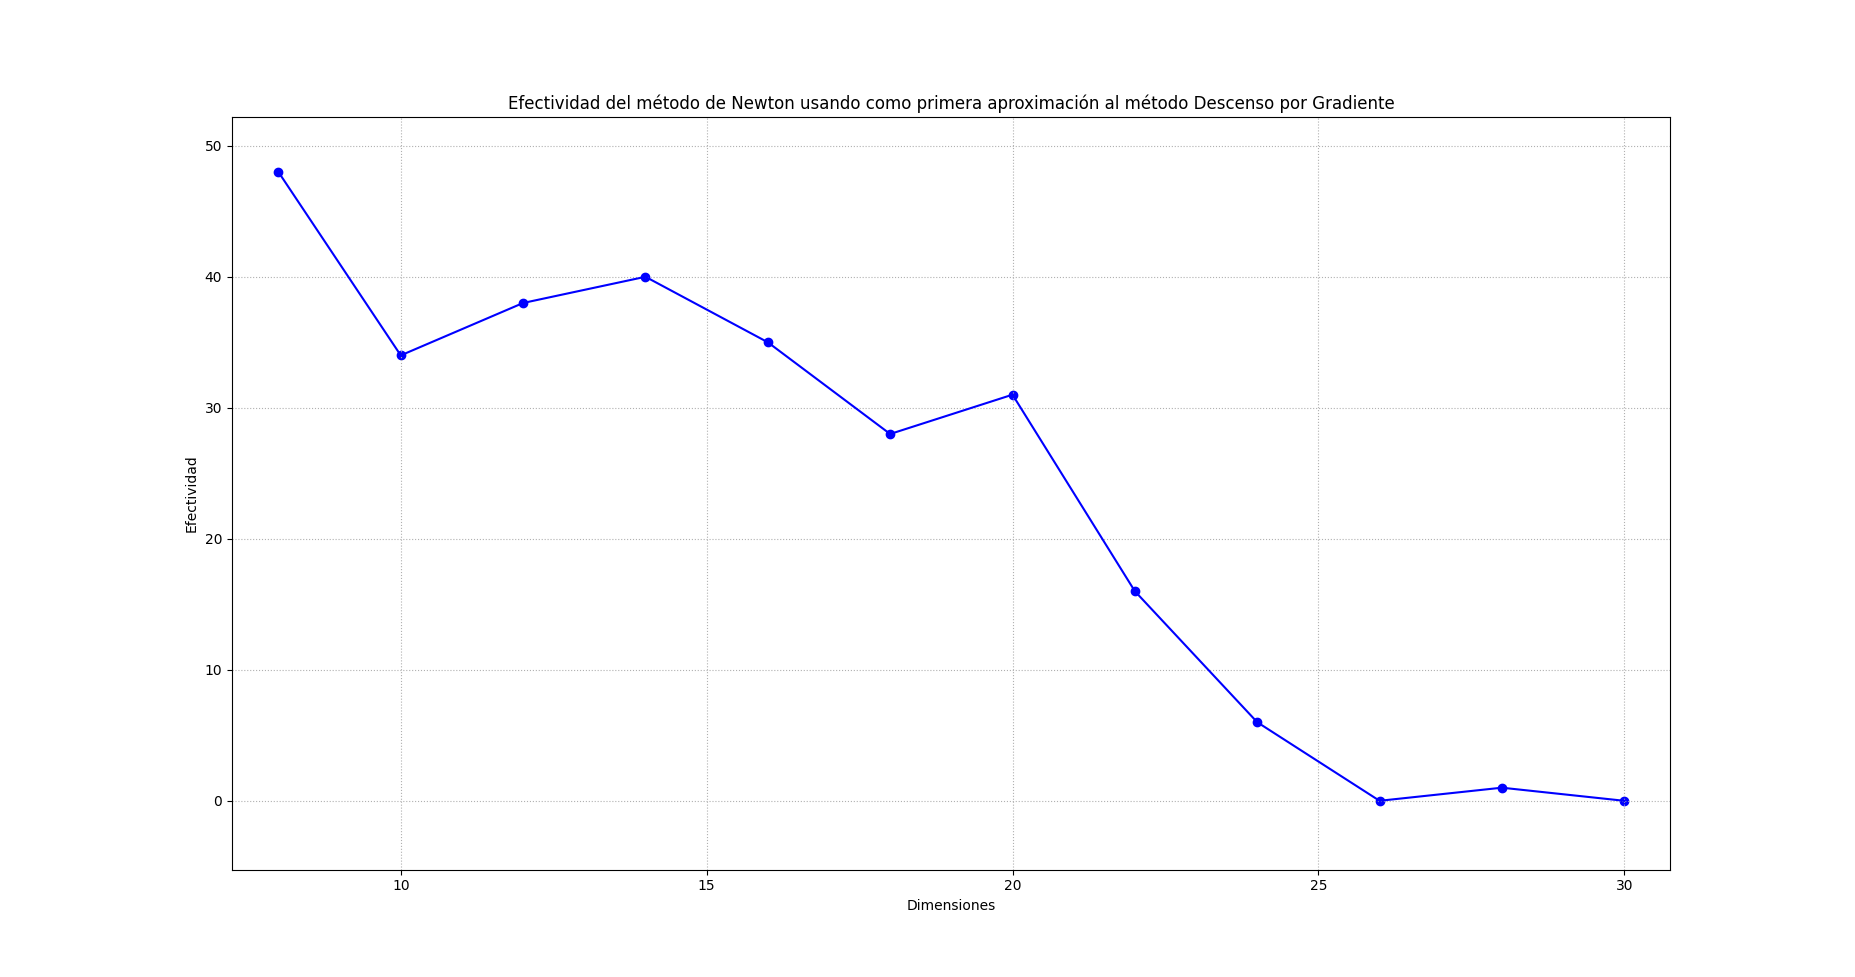
\includegraphics[width=.45\textwidth]{Graphics/GD_N.png}
        \label{GD-N}}
    \subfigure[\begin{scriptsize}
	    Runge-Kutta y Newton
        \end{scriptsize}]{
        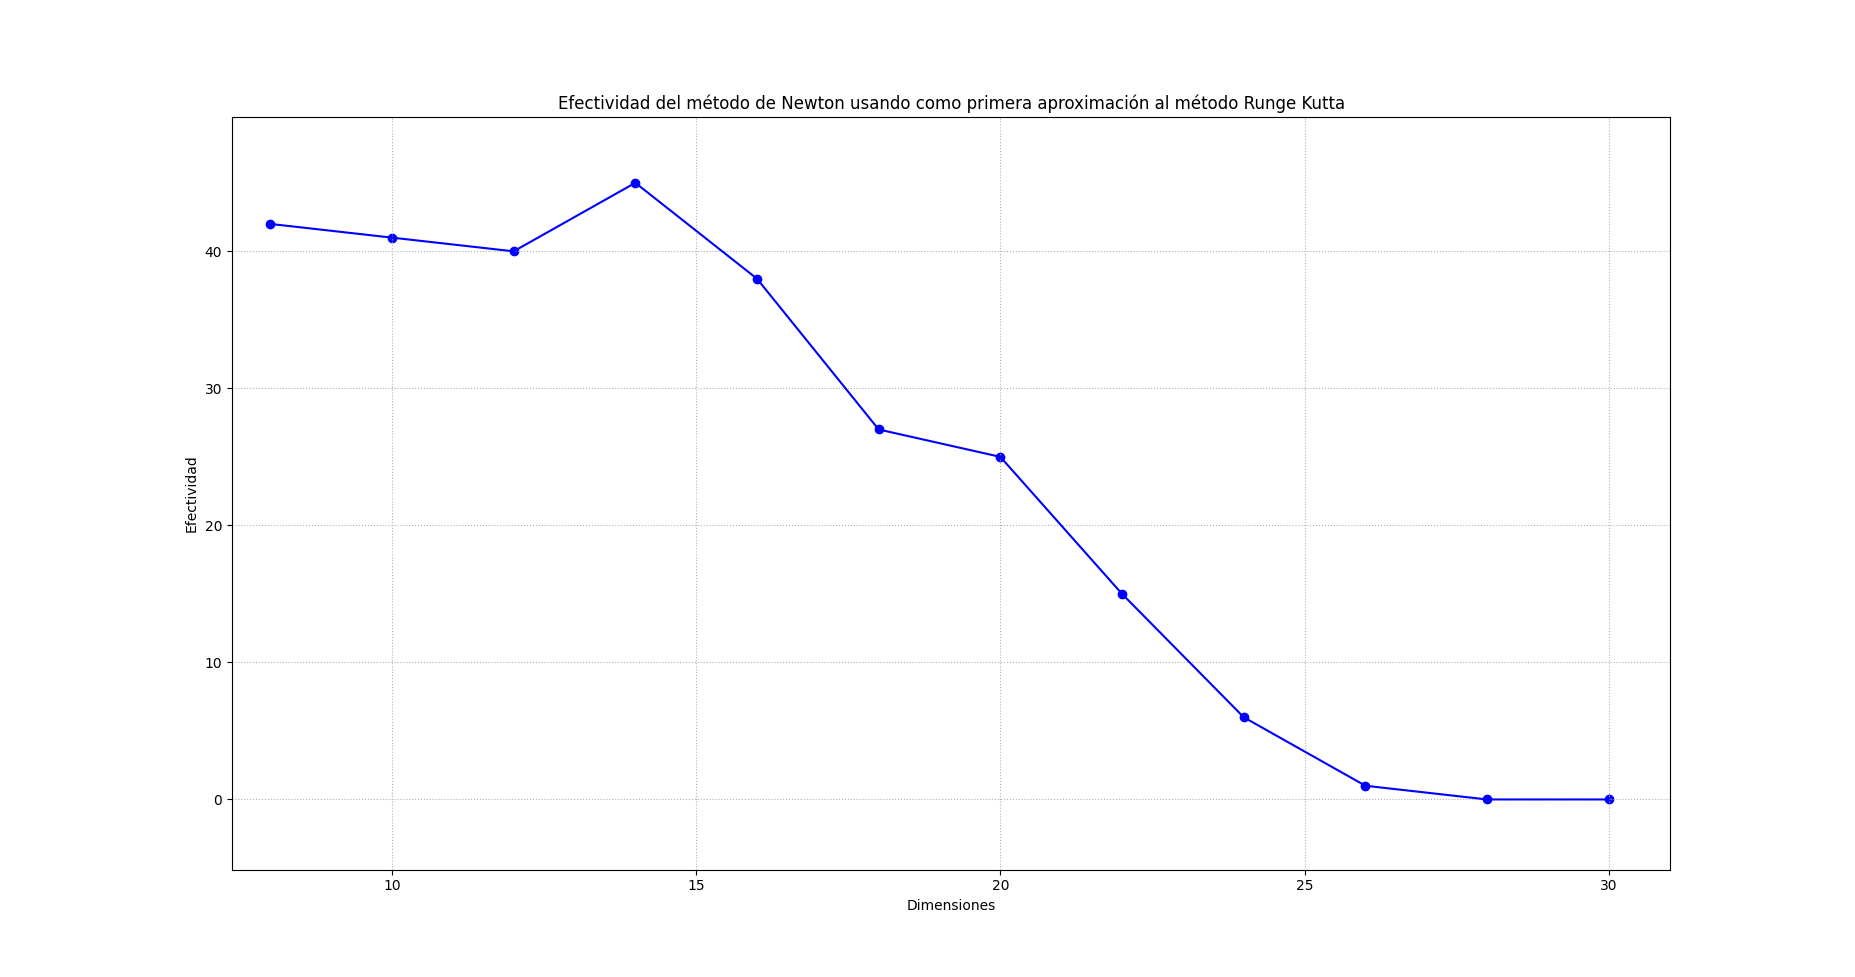
\includegraphics[width=.45\textwidth]{Graphics/RK_N.png}
        \label{RK-N}}
    \subfigure[\begin{scriptsize}
        Descenso por Gradiente y Cuasi-Newton
        \end{scriptsize}]{
        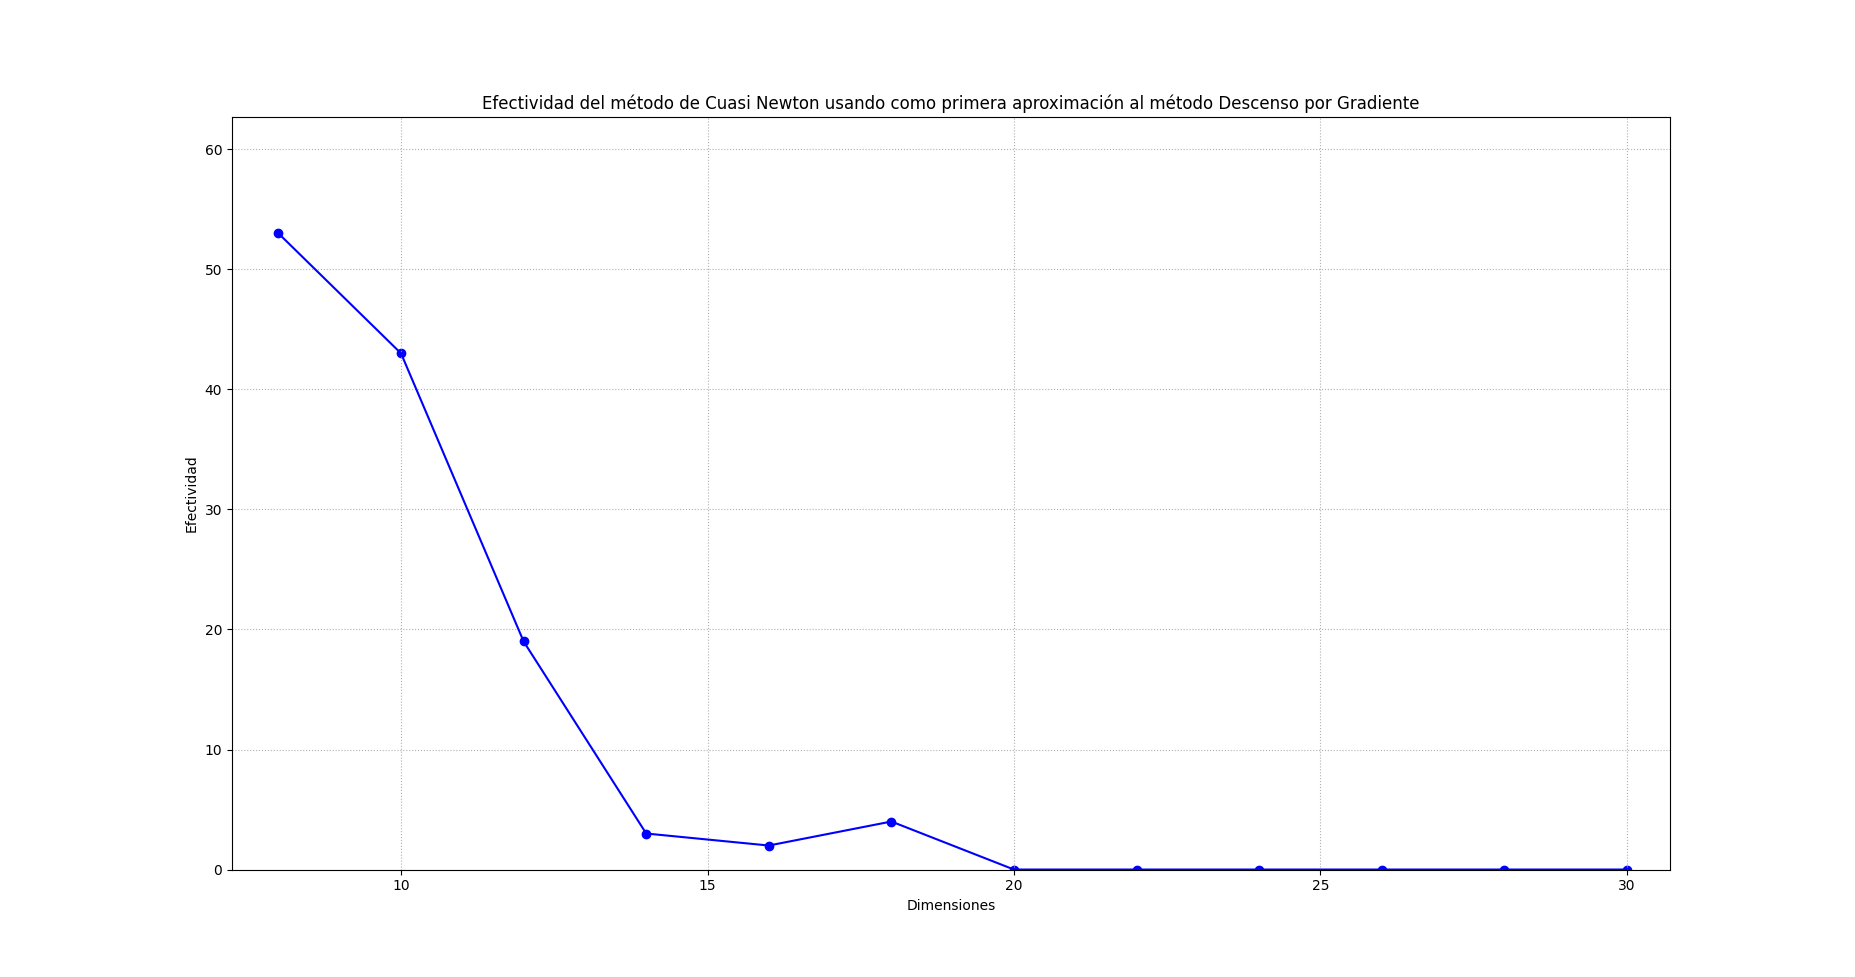
\includegraphics[width=.45\textwidth]{Graphics/GD_CN.png}
        \label{GD-CN}}
    \subfigure[\begin{scriptsize}
        Runge-Kutta y Cuasi-Newton
        \end{scriptsize}]{
        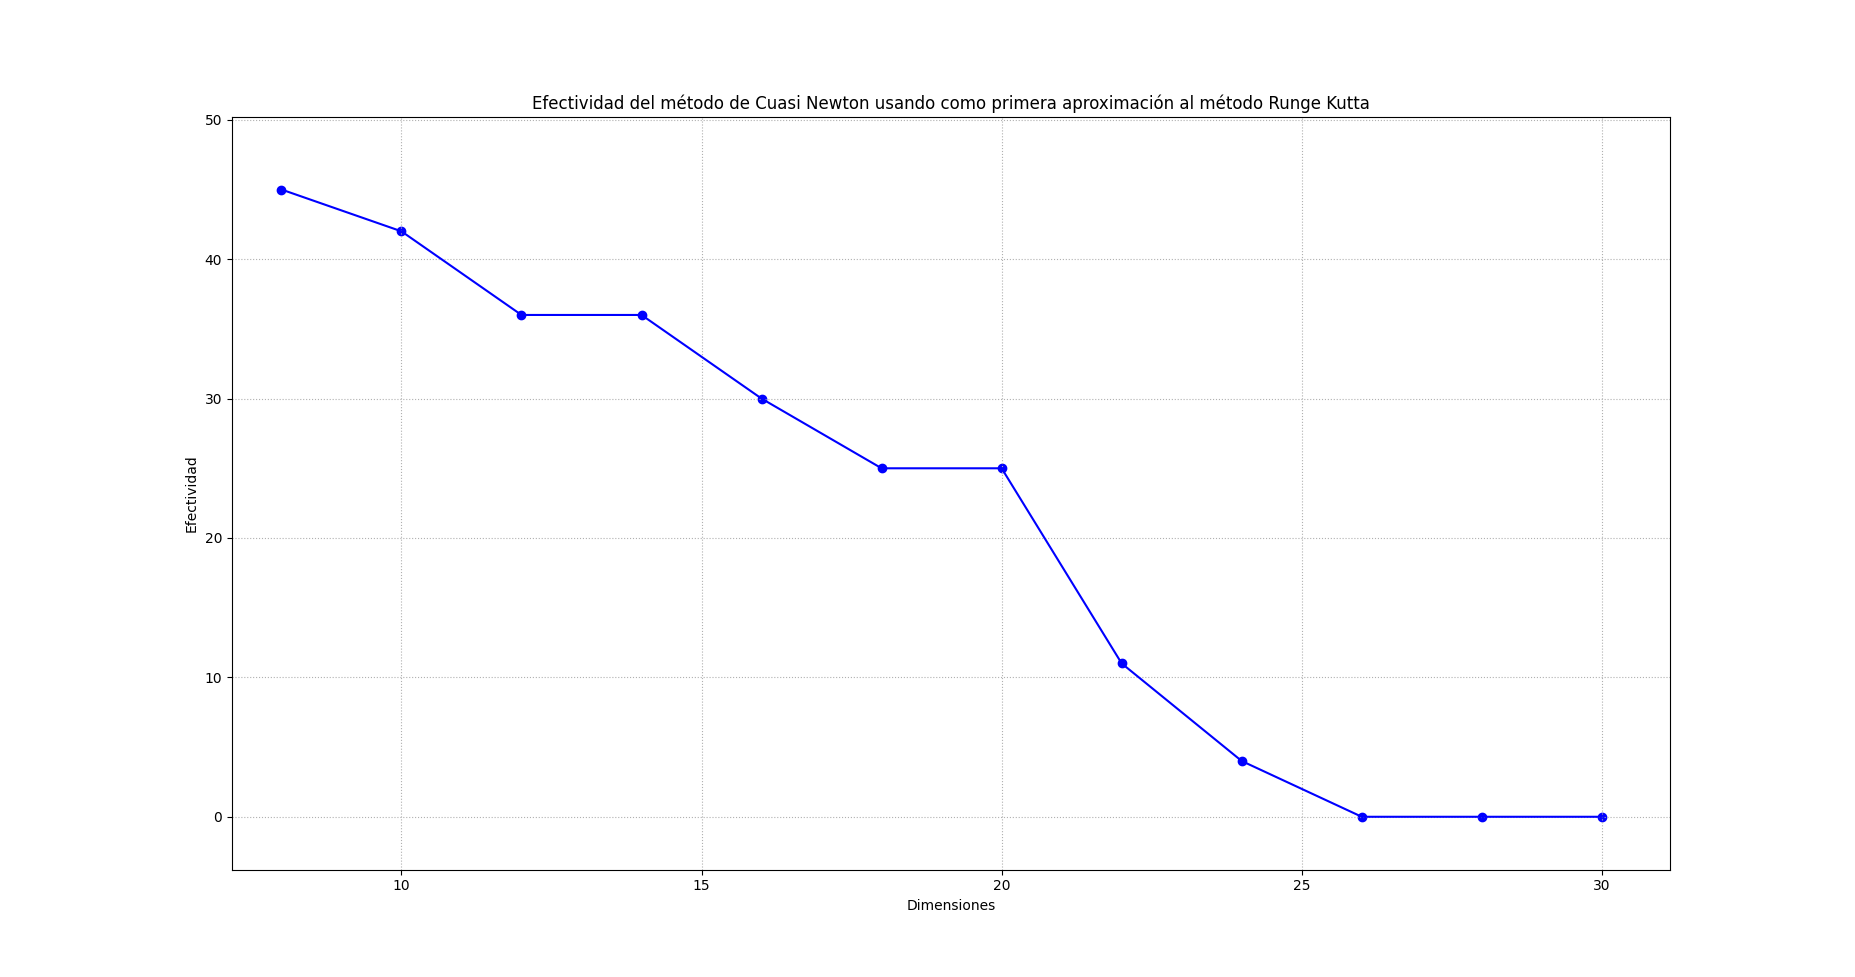
\includegraphics[width=.45\textwidth]{Graphics/RK_CN.png}
        \label{RK-CN}}
    \subfigure[\begin{scriptsize}
        Descenso por Gradiente y Gekko
        \end{scriptsize}]{
        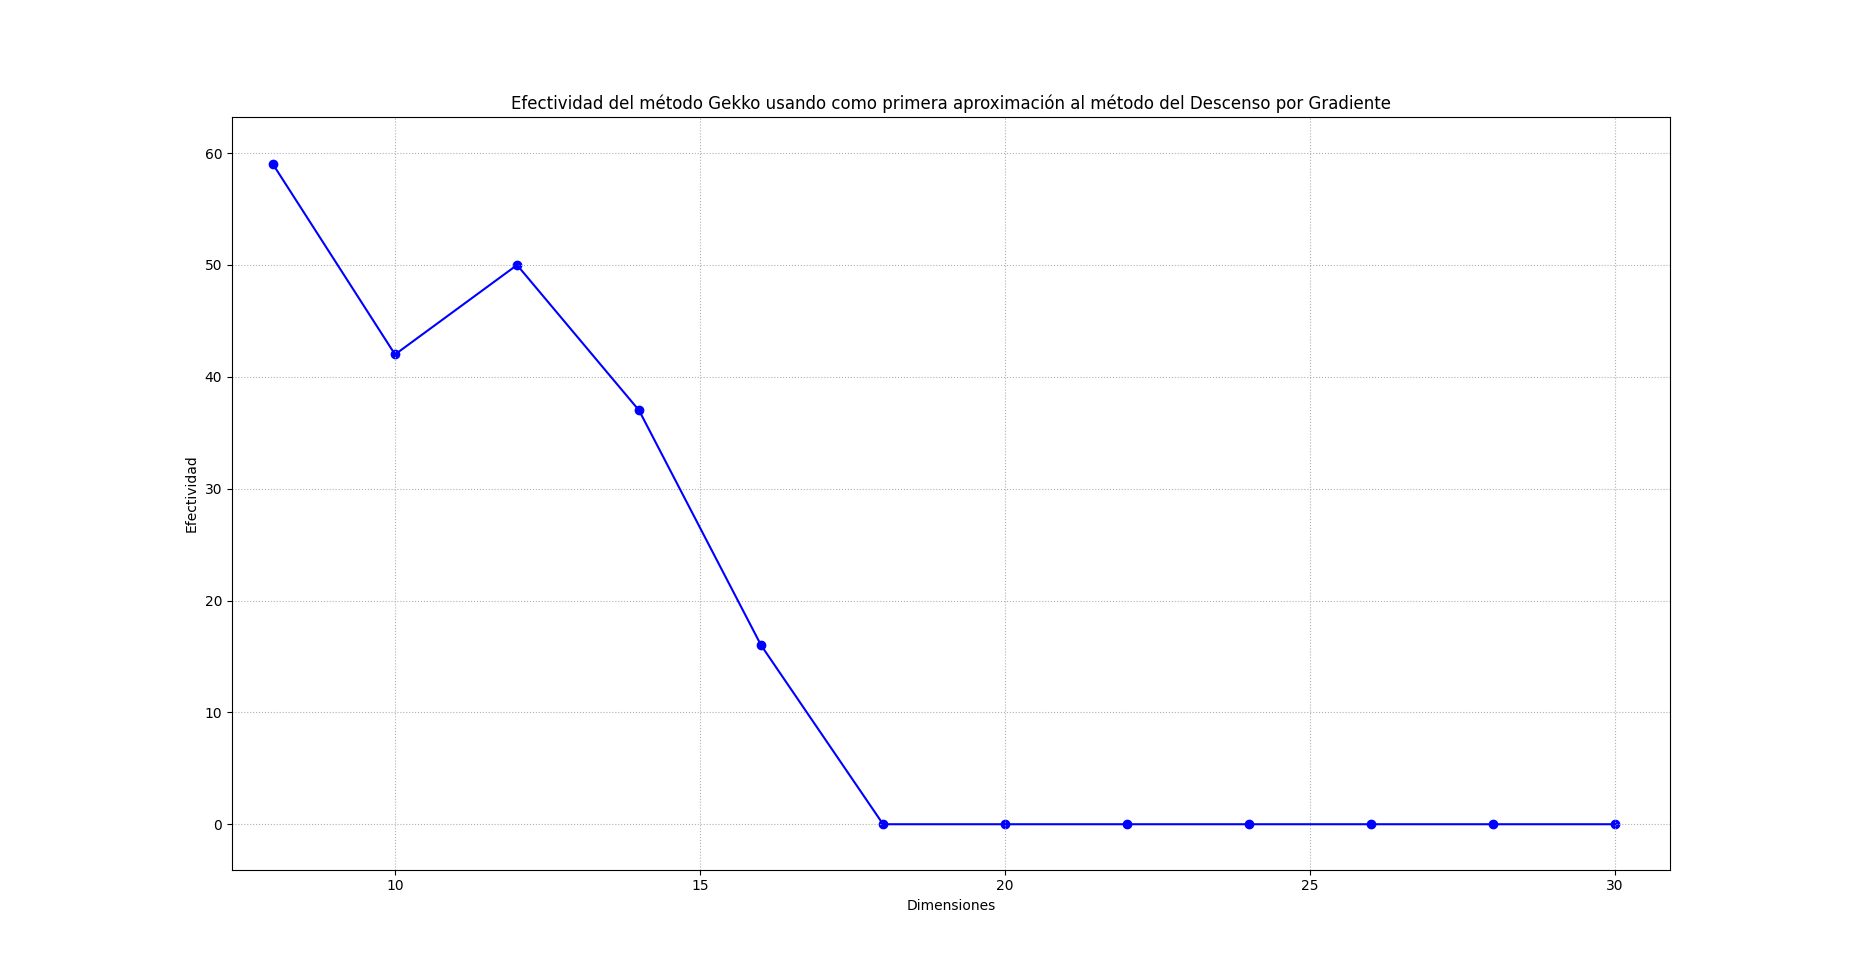
\includegraphics[width=.45\textwidth]{Graphics/GD_Gekko.png}
        \label{GD-G}}
    \subfigure[\begin{scriptsize}
        Runge-Kutta y Gekko
        \end{scriptsize}]{
        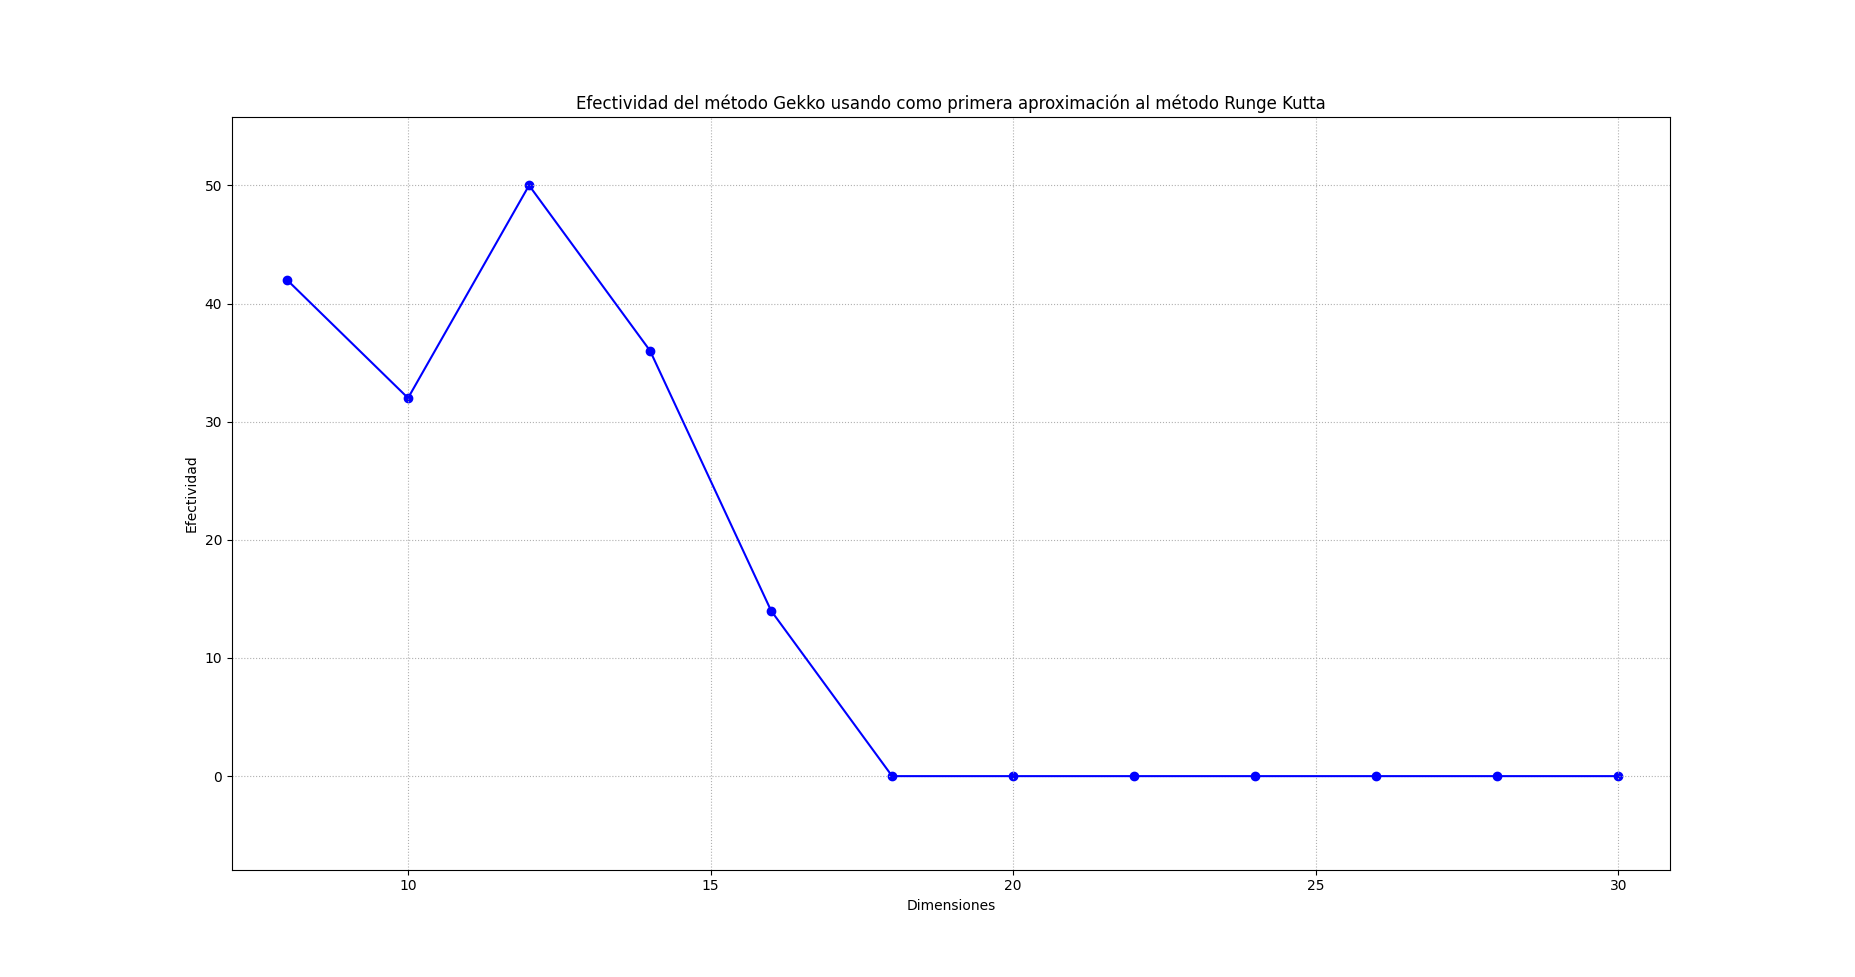
\includegraphics[width=.45\textwidth]{Graphics/RK_Gekko.png}
        \label{RK-G}}
    \caption{Resultados obtenidos empleando los m\'etodos del Descenso por Gradiente y Runge-Kutta para encontrar una aproximaci\'on inicial y, los m\'etodos Newton, Cuasi-Newton y Gekko para resolver el sistema.}
    \label{metodos-combinados}
  \end{center}
\end{figure}

\par Seg\'un los resultados mostrados, Newton con aproximaci\'on inicial a Runge-Kutta constituye la combinaci\'on de m\'etodos con mayor compatibilidad con el sistema propuesto y, por consiguiente, la combinaci\'on que se usar\'a para determinar los filtros de las shapelets, al menos para el caso de una dimensi\'on.\\

\section{Algoritmo de reconocimiento en una dimensi\'on}

\par Una vez se tiene la se\~nal del patr\'on, el primer paso es definir el sistema de ecuaciones a partir del mismo y resolverlo aplicando los m\'etodos de Runge-Kutta y Newton. Al resolver el sistema se obtienen los valores de las componentes del primer vector (llam\'emoslo $v$). A partir de $v$ se construyen los vectores $u$, $\tilde{u}$ y $\tilde{v}$ siguiendo las definiciones dadas en la secci\'on 1.1.1. Con estos cuatro vectores, se construye el banco de filtros y con \'el la wavelet. Para ello, se emplea la biblioteca \textit{PyWavelets} [\cite{27}] de Python, con la cual es posible crear una wavelet recibiendo como par\'ametro el banco de filtros (ver c\'odigo 3.1):\\

\begin{lstlisting}[caption=Creaci\'on de una wavelet a partir del banco de filtros]
shapelet = pywt.Wavelet(filter_bank = [u_, v_, u, v])
\end{lstlisting}

\par El siguiente paso es tomar una se\~nal en la cual se quiere determinar si el patr\'on est\'a o no presente, y aplicar la transformada de wavelet usando la wavelet creada con el filtro:\\

\begin{lstlisting}[caption=C\'alculo de la transformada discreta de Wavelet usando pywt]
cA, cD = pywt.dwt(signal, shapelet)
\end{lstlisting}

para posteriormente determinar, seg\'un los valores cercanos a cero de $cD$, la presencia del patr\'on en la se\~nal.

Consid\'erese el caso de ejemplo de la secci\'on 1.1.3:
\begin{eqnarray}
m=(0.2,0.5,0.45,0.85,0.8,-0.75,0.25,0.2,0.55).\nonumber
\end{eqnarray}

\par Tras construir el sistema y resolverlo se obtiene como una de las posibles soluciones:

\begin{eqnarray}
v=(0.0445, 0.4373, 0.1074, -1.6020, 1.0664, -0.2296, 0.1959, -0.0199),\nonumber
\end{eqnarray}

mientras que:

\begin{eqnarray}
u&=&(0.4373, -0.0445, -0.0199, 0.1959, -0.2296, -1.0664, -1.6020, -0.1074),\nonumber\\
\tilde{v}&=&(0.0445, -0.0199, 0.1959, -0.2296, 1.0664, -1.6020, 0.1074, 0.4373),\nonumber\\
\tilde{u}&=&(0.4373, -0.1074, -1.6020, -1.0664, -0.2296, -0.1959, -0.0199, -0.0445).\nonumber
\end{eqnarray}

\par Notar que los valores obtenidos son completamente distintos a los del ejemplo de la secci\'on 1.1.3, sin embargo, al comprobar las condiciones de la 1.1-1.5 se cumplen todas. Con los cuatro vectores anteriores se crea el banco de filtros $[\tilde{u},\tilde{v},u,v]$ y se construye la shapelet.\\

\par Al procesar la se\~nal de muestra definida tambi\'en en el ejemplo anterior, se obtiene el gr\'afico de valores de $cD$ mostrado en la Figura 3.7, en el cual se puede apreciar que el pico que indica la detecci\'on del patr\'on se encuentra en la posici\'on $24$.

\begin{figure}[h]
\center
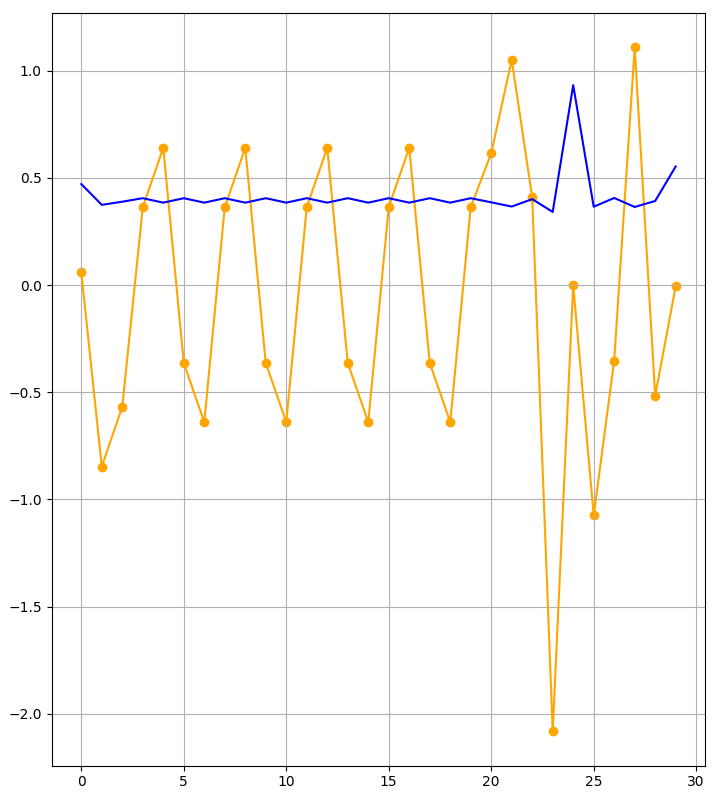
\includegraphics[width=50mm,height=45mm]{Graphics/patternDetected1D.png}
\caption{Vector $cD$ obtenido tras aplicar la DST (naranja) y la medida de similaridad con $\alpha=0.1$ (azul).}
\end{figure}

\par Como se cumple que:
\begin{eqnarray}
cD(n)=0&\Leftrightarrow& D(f\ast\tilde{v})(n)=0\nonumber\\
&\Leftrightarrow&(f\ast\tilde{v})(2n)=0\nonumber\\
&\Leftrightarrow&\sum_{m=0}^{N-1}v(m)f(2n-m)=0,\nonumber
\end{eqnarray}
entonces, si $cD(n)=0$ el patr\'on se encuentra contenido en $f$ en el intervalo $[2n-N+1,2n]$, por tanto, tomando $n=24$, se cumple que $2n-N+1=41$ es la posici\'on exacta en la que comienza el patr\'on dentro de la se\~nal.

\par Como parte del an\'alisis del programa se generaron varios patrones de forma aleatoria con dimensi\'on tambi\'en variable y se insertaron dentro de una se\~nal en una posici\'on aleatoria con una probabilidad de $0.5$. Sin embargo, el patr\'on fue detectado satisfactoriamente en el $100\%$ de los casos que aparec\'ia, al igual que la detecci\'on de la ausencia en el $100\%$ de los casos en los que no se incluy\'o el patr\'on en la se\~nal.\\

\par Como un segundo experimento, se generaron $676$ casos de prueba con patr\'on aleatorio e inclusi\'on aleatoria en la se\~nal, pero esta vez con un ruido en el orden $10^{-3}$.  La Figura 3.8 muestra los gr\'aficos de precisi\'on y recobrado del algoritmo durante el proceso de detecci\'on de la presencia o no del patr\'on en dependencia del umbral usado para la medida de similiaridad.

\begin{figure}[h]
\center
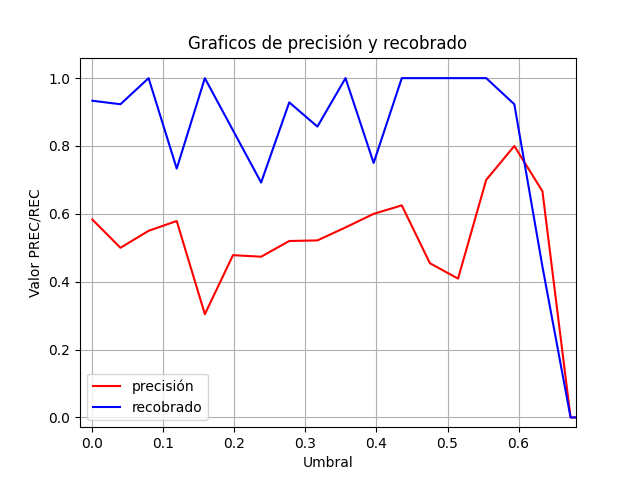
\includegraphics[scale=.45]{Graphics/PrecRec1D.png}
\caption{Precisi\'on y Recobrado del algoritmo de una dimensi\'on para distintos valores del umbral usando la mediada $\mathbb{S}$.}
\end{figure}

\par Note que, aun con la presencia de ruido en el patr\'on dentro de la se\~nal, se muestra un valor de precisi\'on y recobrado aceptable. Como un \'ultimo experimento, se usaron otras bases wavelets (las mencionadas al final de la secci\'on 1.1.3) para intentar detectar el patr\'on sin \'exito alguno. La raz\'on de esto se debe a que ninguna de estas wavelets tiene en cuenta el patr\'on que se desea localizar, por tanto, no se puede esperar obtener un comportamiento distinto para distintos casos de patrones que se incluyan en una se\~nal.

\section{Algoritmo de reconocimiento en dos dimensiones}

\par El problema principal, es crear una base wavelet que permita reconocer anomal\'ias en una mamograf\'ia digital. Para ello, tanto la mamograf\'ia como la anomal\'ia son representadas como im\'agenes con la particularidad de que esta \'ultima debe tener iguales proporciones de ancho y altura. Estas im\'agenes que representan los datos a procesar se encuentran en formato \texttt{.dcm}, tambi\'en conocido como im\'agenes DICOM. Este es un formato internacional que se desarrolló con el fin de almacenar las imágenes del cuerpo tomadas con equipos de imágenes médicas. Incluye imágenes de resonancia magnética y tomografía por ordenador, imágenes de ultrasonido, mamograf\'ias, entre otras, en una escala real. DCM también almacena la información del paciente en los metadatos, que forman parte de un único archivo.\\

\par En el software desarrollado se emplea la biblioteca \textit{Pydicom} [\cite{15}], creada espec\'ificamente para el trabajo con archivos de tipo \texttt{dcm}. Sup\'ongase que se desea leer primeramente la imagen de la anomal\'ia que a su vez constituye el patr\'on, usando \textit{pydicom} ser\'ia tan simple como ejecutar:\\
\begin{lstlisting}[caption=Leer una imagen .dcm., label=pydicom-read]
ds = pydicom.dcmread(path, force=True)
\end{lstlisting}
con lo cual se lee la imagen de la direcci\'on \texttt{path} y se almacena en \texttt{ds} como un archivo de tipo \texttt{pydicom.FileDataset}. De aqu\'i, lo m\'as relevante, es el valor de \texttt{ds.pixel\_array}, que contiene la matriz de valores de los p\'ixeles de la mamograf\'ia.\\

\par El siguiente paso, es crear el sistema de ecuaciones no lineales. Y aqu\'i una nota muy importante, aunque el m\'etodo de Newton usado con Runge-Kutta mostr\'o mejores resultados en el caso de una dimensi\'on, al incluir dos ecuaciones nuevas con una cantidad de $N^2$ t\'erminos, el m\'etodo de Newton comienza a presentar dificultades para resolver el sistema, mientras que por otro lado, Gekko muestra un buen desempe\~no con el aumento de t\'erminos, esto se debe a que dicha biblioteca posee su propio m\'etodo de representar los datos. Entonces, dado que ambos m\'etodos (Gekko y Runge-Kutta) requieren una representaci\'on distinta de los datos, existen dos formulaciones del modelo en el programa. El primero de ellos (Runge-Kutta) usa la funci\'on multivariable como la funci\'on a la cual se le quiere hallar la ra\'iz y el jacobiano del sistema. Para esto se crearon dos funciones: \texttt{func} y \texttt{jac} que retornan la evaluaci\'on de la funci\'on multivariable y el jacobiano en un punto dado, respectivamente. Para mejorar la eficiencia del programa, se plante\'o el sistema en forma matricial usando la biblioteca de Python: \textit{numpy} [\cite{14}], de esta forma evaluar cada funci\'on en un valor del dominio se transforma en operaciones entre matrices \textit{numpy}, que se realizan en un tiempo mucho menor en comparaci\'on a las operaciones con matrices en Python.
\par Por su parte, Gekko usa las ecuaciones en su representaci\'on algebraica, esto es plantear las ecuaciones tal y como se plantearon en (1.1)-(1.5), una vez hecho se definen las opciones de resoluci\'on del sistema y, por \'ultimo, se invoca al m\'etodo \texttt{solve()} para encontrar la soluci\'on.\\

\par Tras construir la wavelet con el banco de filtro hallado, se procede a cargar la imagen de prueba usando \textit{pydicom} como se muestra en el ejemplo de c\'odigo~\ref{pydicom-read}. De la imagen se extrae la matriz de valores de los p\'ixeles y se le aplica la transformada wavelet de dos dimensiones.
\par N\'otese algo muy importante, en las mamograf\'ias digitales predominan los valores 0, que representan el color negro en la escala de grises, al aplicar la transformada de wavelets en dos dimensiones usando \textit{PyWavelets}, en alg\'un punto se calcula la convoluci\'on entre el filtro y una secuencia de ceros en la imagen, lo cual va a resultar en un valor igual a cero en la matriz de detalle. Dado que se usa la cercan\'ia a este valor como medida de similaridad entre el patr\'on y el fragmento de la muestra, podr\'ia representar un problema, llegando a producir un gran n\'umero de falsos positivos.
\par Para evitar este inconveniente se calcula la transformada wavelet de forma manual, as\'i, si en alg\'un punto se calcula la convoluci\'on entre el vector $\tilde{v}$ del filtro y una secuencia de al menos $\frac{N^2}{4}$ ceros, no se considera el resultado obtenido como posible ocurrencia del patr\'on.\\

\par Al aplicar entonces la transformada wavelet se obtienen las matrices \texttt{cA}, \texttt{cH}, \texttt{cV} y \texttt{cD}. De ellas se toma la \'ultima y se realiza la b\'usqueda de ceros que indiquen la ocurrencia del patr\'on. Sup\'ongase que se encuentra una posible ocurrencia del patr\'on en $(i,j)$, realizando el mismo an\'alisis que en una dimensi\'on, se tiene:
\begin{eqnarray}
cD(i,j)=0&\Leftrightarrow&D(img\ast\tilde{w}_{0,0})(i,j)=0\nonumber\\
&\Leftrightarrow&(img\ast\tilde{w}_{0,0})(2i,2j)=0\nonumber\\
&\Leftrightarrow&\sum_{n=0}^{N-1}\sum_{m=0}^{N-1}\tilde{w}_{0,0}(n,m)img(2i-n,2j-m)=0,\nonumber
\end{eqnarray}
cuyo resultado indica la ocurrencia del patr\'on entre $(2i-N+1,2j-N+1)$ y $(2i,2j)$.

\par Un punto muy importante que se tiene en cuenta es la ocurrencia del patr\'on en una imagen con ruido. En estos casos es casi imposible lograr una medida $\mathbb{S}$ cercana a la unidad, por esta raz\'on se emplea un umbral de detecci\'on, de esta forma, cualquier valor en la medida $\mathbb{S}$ que sobrepase este umbral es considerada una ocurrencia del patr\'on, mientras que, de quedar por debajo, se considera que el patr\'on no se localiz\'o en la posici\'on actual.\\

\par Para analizar el funcionamiento del algoritmo se mostrar\'a un ejemplo con im\'agenes. Suponga que se desea reconocer la ocurrencia de una letra (digamos \texttt{c}, ver Figura~\ref{img-ejemplo}) en una lista de palabras:

\begin{figure}[h]
\center
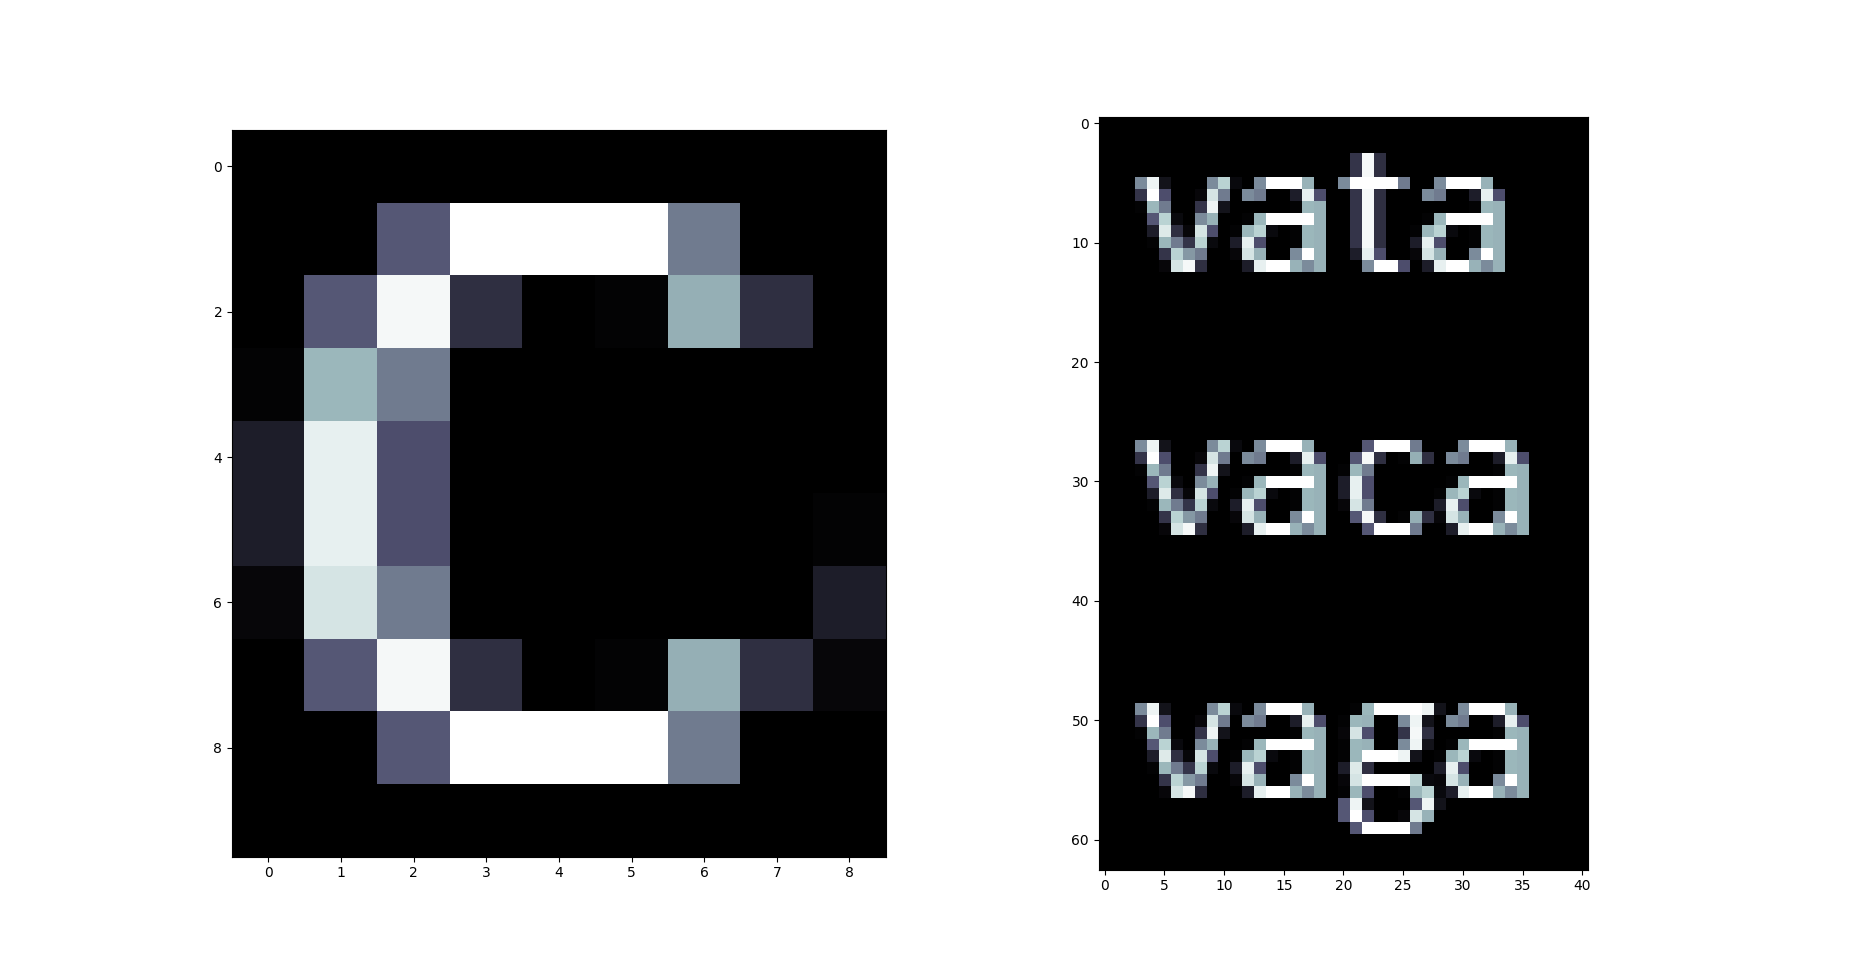
\includegraphics[scale=.2]{Graphics/cWordList.png}
\caption{Ejemplo de un patr\'on y una imagen de prueba.}
\label{img-ejemplo}
\end{figure}

\par Para este caso se toma $N=8$ como la dimensi\'on de los vectores del filtro. Tras leer la imagen con \textit{PyWavelets}, se obtiene la siguiente representaci\'on matricial:
\begin{scriptsize}
\begin{eqnarray}
m&=&\left[\begin{array}{rrrrrrrrr}
0&0&0&0&0&0&0&0&0\\
0&0&0.0015&0.0039&0.0039&0.0039&0.002&0&0\\
0&0.0015&0.0038&0.0008&0&0.0001&0.0026&0.0008&0\\
0.0001&0.0027&0.002&0&0&0&0&0&0\\
0.0005&0.0036&0.0014&0&0&0&0&0&0\\
0.0005&0.0036&0.0014&0&0&0&0&0&0.0001\\
0.0001&0.0034&0.002&0&0&0&0&0&0.0005\\
0&0.0015&0.0038&0.0008&0&0.0001&0.0026&0.0008&0.0001\\
0&0&0.0015&0.0039&0.0039&0.0039&0.002&0&0\\
0&0&0&0&0&0&0&0&0
\end{array}\right].\nonumber
\end{eqnarray}
\end{scriptsize}

\par Con los valores de esta matriz se construyen las ecuaciones de detecci\'on y junto con el resto de las condiciones se forma el sistema de ecuaciones. A la hora de resolverlo se usa primeramente una aproximaci\'on inicial a la r\'aiz proporcionado por el m\'etodo de Runge-Kutta. Los valores $x_0$ son generados de forma aleatoria y por tanto la ra\'iz encontrada en cada ejecuci\'on podr\'ia cambiar. Por ejemplo, en este caso, antes de aplicar Runge-Kutta:
\begin{eqnarray}
x_0&=&(0.773,0.7211,0.382,0.0948,0.0963,0.963,0.2968,0.1797),\nonumber
\end{eqnarray}
mientras que, al aplicar Runge-Kutta se tiene:
\begin{eqnarray}
x_{\ast}&=&(-0.0607,-2.5645,4.3419,14.4576,-0.7601,-21.0409,-2.3254,-8.2964),\nonumber
\end{eqnarray}
el valor de $x_{\ast}$ es usado entonces como valor inicial al aplicar el m\'etodo de \textit{Gekko}. Tras resolver el sistema nuevamente se obtiene:
\begin{eqnarray}
v&=&(0.0061,-0.0121,-0.0813,-0.0222,0.6232,-0.7612,0.141,0.0708).\nonumber
\end{eqnarray}
\par A partir del valor de $v$ obtenido, se calculan el resto de los vectores que conformar\'an el banco de filtros:
\begin{eqnarray}
u&=&(-0.0121,0.0061,0.0708,-0.141,-0.7612,-0.6232,-0.0222,0.0813),\nonumber\\
\tilde{v}&=&(0.0061,0.0708,0.141,-0.7612,0.6232,-0.0222,-0.0813,-0.0121),\nonumber\\
\tilde{u}&=&(-0.0121,0.0813,-0.0222,-0.6232,-0.7612,-0.141,0.0708,0.0061),\nonumber
\end{eqnarray}
con el cual se construye la shapelet.\\

\begin{figure}[h]
\center
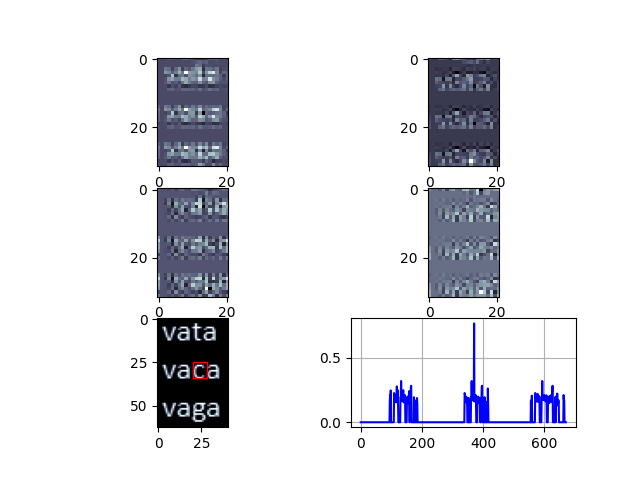
\includegraphics[scale=.7]{Graphics/CDetect.png}
\caption{Imagenes de aproximaci\'on, detalles horizontales, detalles verticales, detalles (com\'unmente llamados diagonales), imagen con el patr\'on se\~nalado y medida $\mathbb{S}$, en ese orden.}
\label{c-detected}
\end{figure}

\par Para el paso de an\'alisis de la imagen en busca de la ocurrencia del patr\'on, se carga el archivo de la misma a partir de su direcci\'on tal como se muestra en el Ejemplo de c\'odigo~\ref{pydicom-read}. Una vez se tiene la forma matricial de la imagen de muestra, se determina la transformada wavelet de dos dimensiones usando la shapelet creada. La Figura~\ref{c-detected} muestra las im\'agenes obtenidas tras aplicar las transformadas junto con los valores de la medida $\mathbb{S}$ para $\alpha=0.1$ aplicada a la matriz \texttt{cD}.

\par Como se puede apreciar hay una amplia diferencia entre la medida $\mathbb{S}$ del punto en el que coincide el patr\'on y el resto de los puntos. Este ejemplo muestra un buen comportamiento del algoritmo, por ello se pasar\'a a analizar que ocurrir\'ia en casos m\'as complejos como es el de detectar tumores en mamograf\'ias.\\

\par Para el siguiente ejemplo, se tom\'o una anomal\'ia y, aplicando la transformada wavelet de Haar, se le redujo la dimensi\'on hasta tener proporciones menores o iguales que una imagen de $26\times 26$ p\'ixeles. La raz\'on se debe a la efectividad mostrada por los m\'etodos de resoluci\'on de sistemas de ecuaciones no lineales ante un aumento del n\'umero de variables. Posteriormente, se determin\'o la shapelet asociada al patr\'on. Luego, se tom\'o una mamograf\'ia digital con el tumor, se redujo sus dimensiones usando el mismo m\'etodo que para el patr\'on un n\'umero igual de veces y, se le aplic\'o la transformada usando la shapelet antes creada. La Figura~\ref{detect-anomalia} muestra los resultados obtenidos en el proceso de detecci\'on.

\begin{figure}[h]
\center
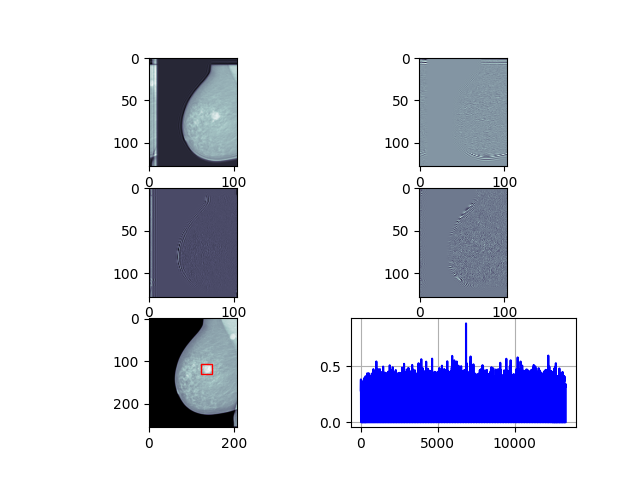
\includegraphics[scale=.7]{Graphics/MamografiaDetect.png}
\caption{Resultados obtenidos en el proceso de detecci\'on de la anomal\'ia en la mamograf\'ia.}
\label{detect-anomalia}
\end{figure}

\par En un segundo ejemplo, se muestra una mamograf\'ia con una anomal\'ia de distinto tama\~no a la anterior y el resultado que se obtiene al ejecutar el algoritmo. Tal como se puede observar en la Figura~\ref{detect-anomalia-piece}, el algoritmo detecta la ocurrencia del patr\'on con una similitud de m\'as del $40\%$, sin embargo, la anomal\'ia es mayor a la del patr\'on empleado, por lo que solo es posible reconocer una peque\~na parte de esta.

\begin{figure}[h]
\center
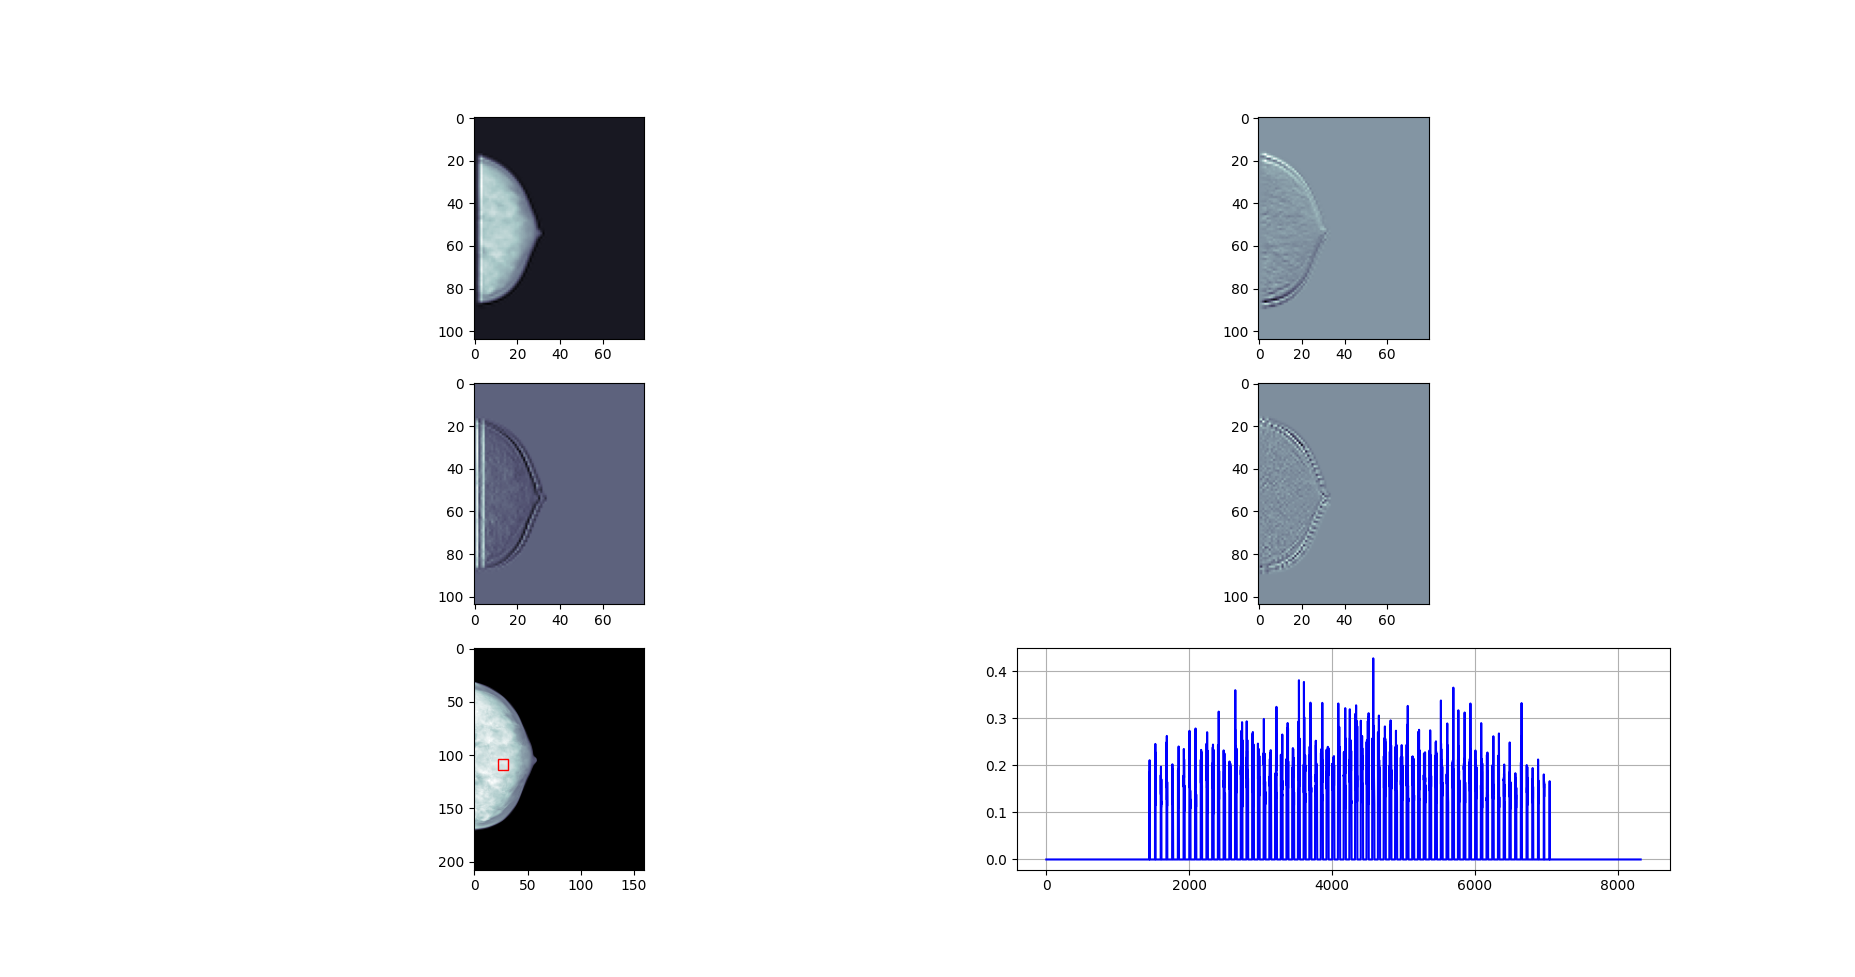
\includegraphics[scale=.32]{Graphics/MamografiaDetectPiece.png}
\caption{Resultados obtenidos en el proceso de detecci\'on de la anomal\'ia irregular en la mamograf\'ia.}
\label{detect-anomalia-piece}
\end{figure}

\par Como tercer ejemplo, se tom\'o una mamograf\'ia sin anomal\'ias, pero, debido a las caracter\'isticas de la imagen, el algoritmo produjo un falso positivo como se muestra en la Figura~\ref{detect-anomalia-fail}. La textura de una im\'agen puede variar en dependencia del equipo con el cual se haya tomado la muestra y, puede repercutir positiva o negativamente en el proceso de reconocimiento.

\begin{figure}[h]
\center
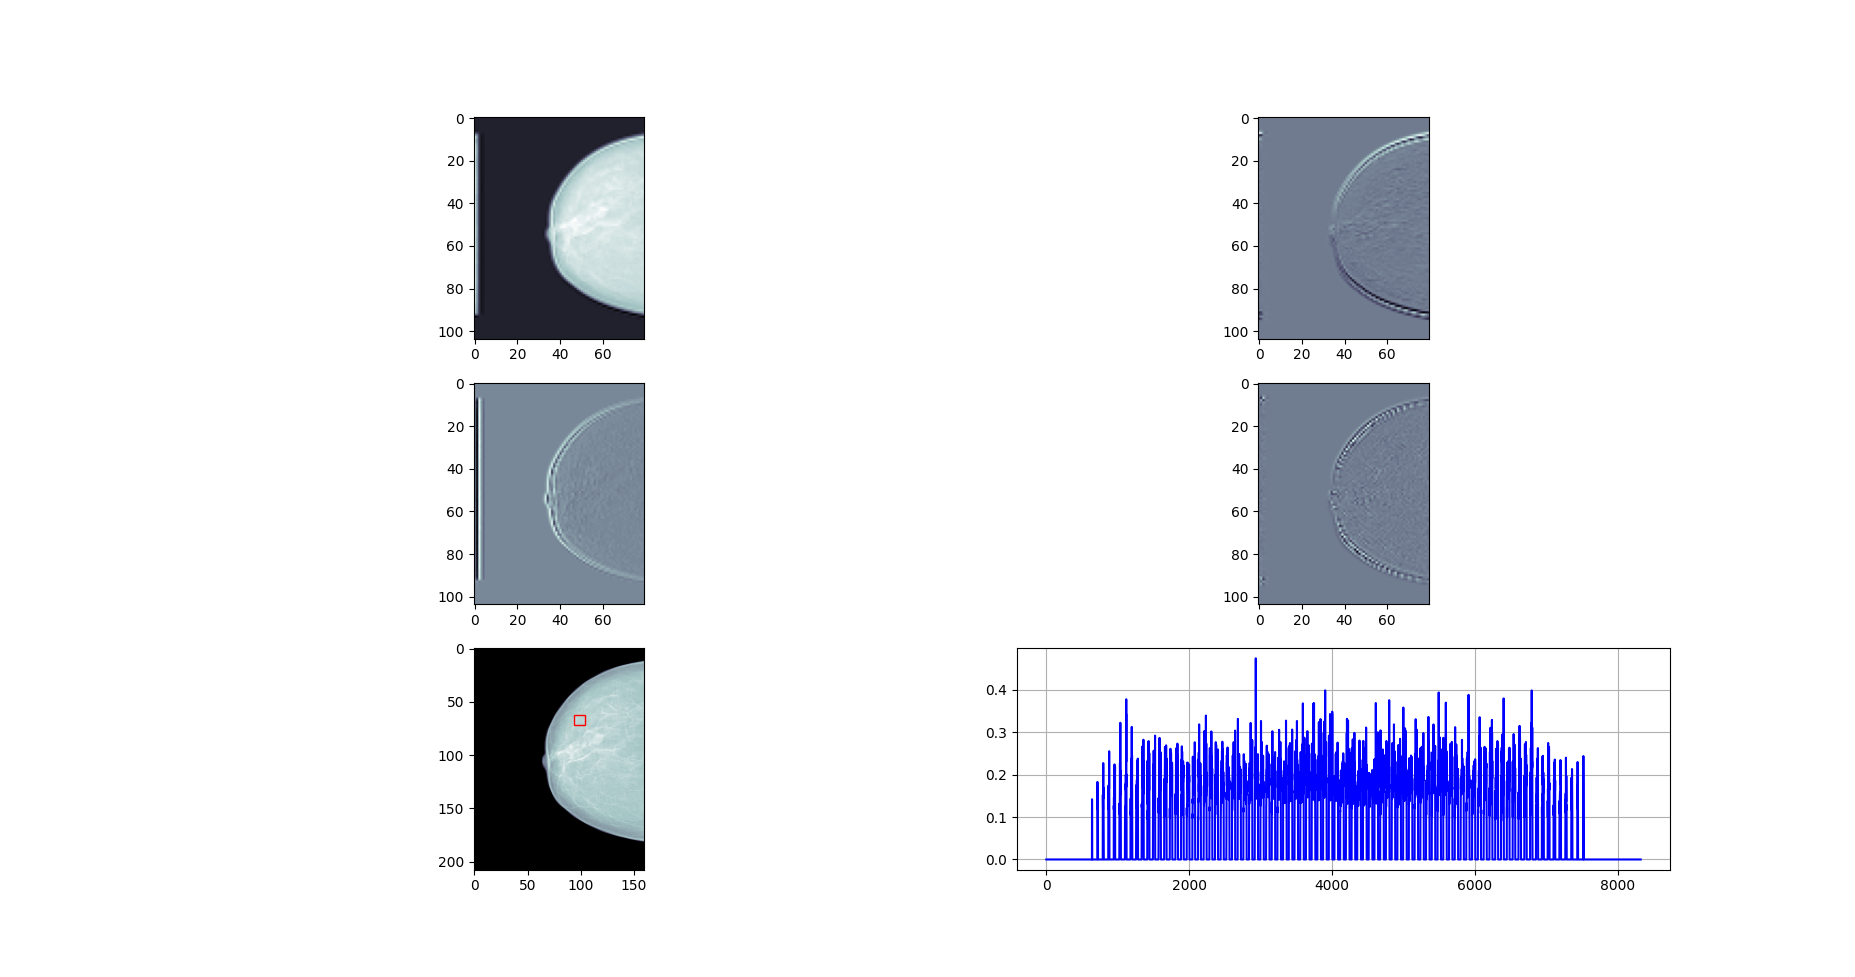
\includegraphics[scale=.32]{Graphics/MamografiaDetectFail.png}
\caption{Resultados obtenidos en el proceso de reconocimiento en una imagen sin anomal\'ias.}
\label{detect-anomalia-fail}
\end{figure}

\par Para poner a prueba el algoritmo, se tom\'o una colecci\'on de mamograf\'ias digitales tanto de personas sanas, como de personas con c\'ancer y con presencia de un posible tumor. Se tom\'o un patr\'on de una anomal\'ia, se cre\'o la sheplet correspondiente y, posteriormente, se ejecut\'o el algoritmo para cada imagen de muestra. La Figura~\ref{prec-rec-2d} muestra los valores de precisi\'on y recobrado para un aumento de los casos de prueba.

\begin{figure}[h]
\center
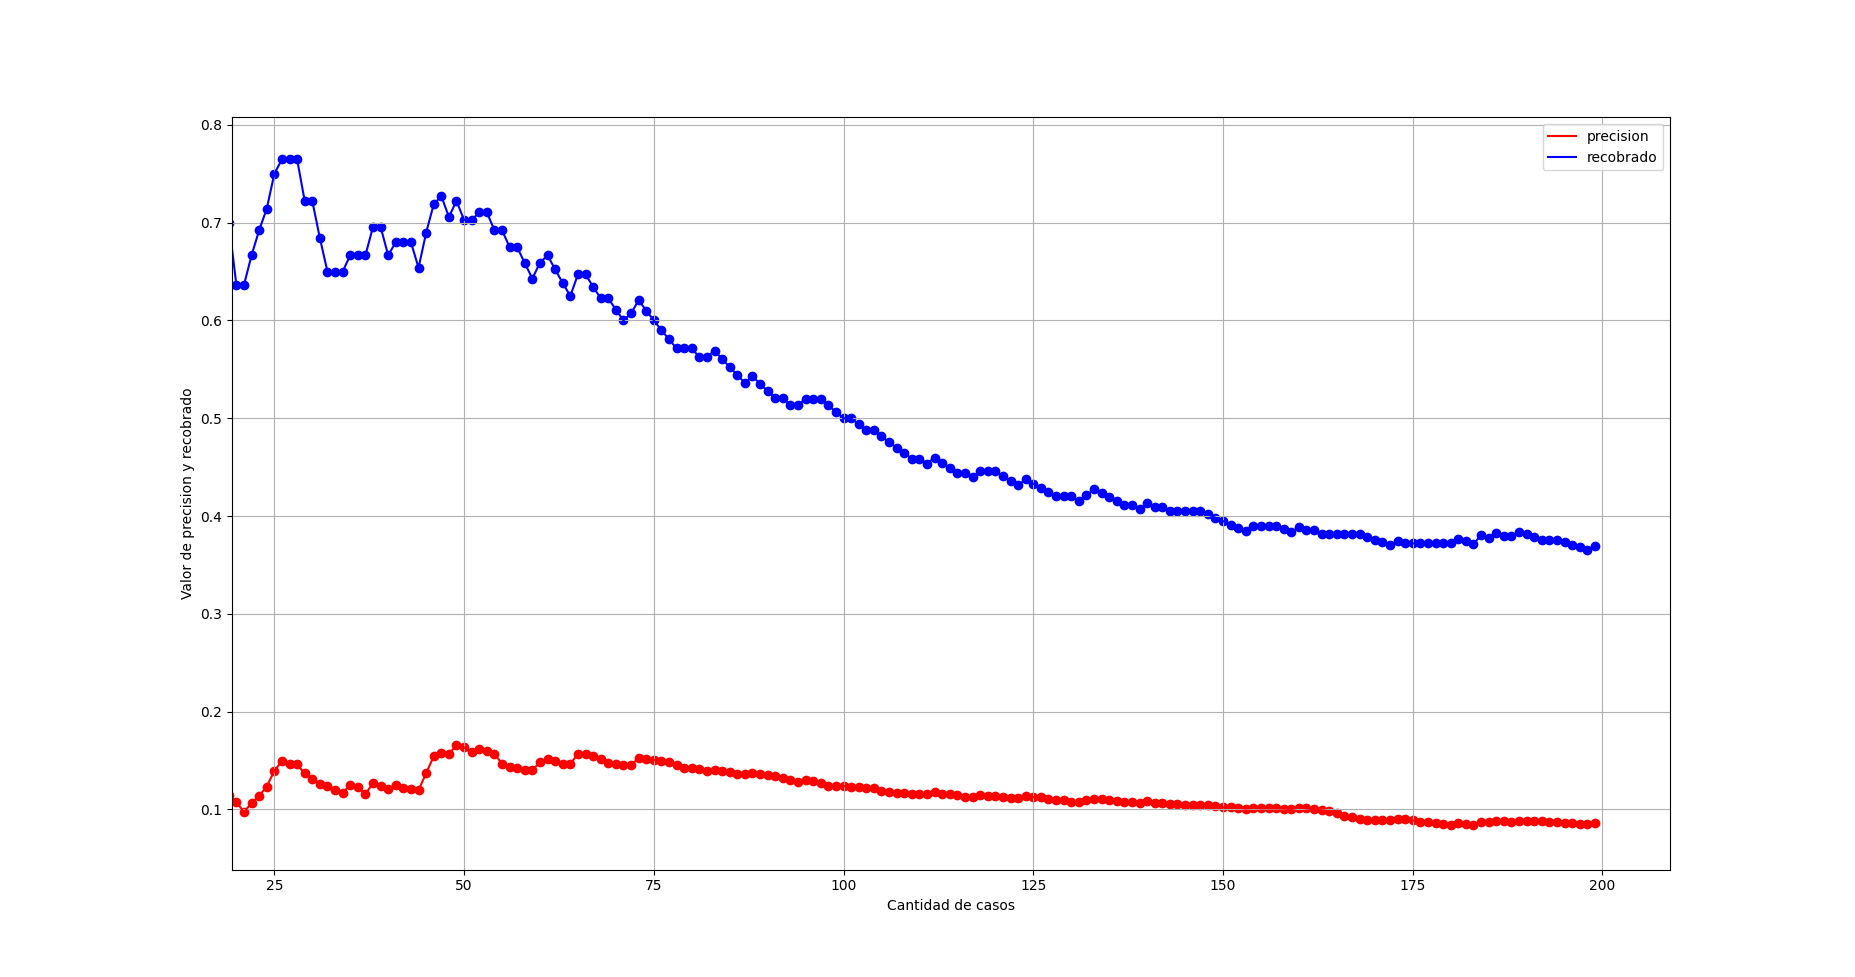
\includegraphics[scale=.25]{Graphics/PrecRec2D.png}
\caption{Valores de precisi\'on y recobrado obtenidos durante el aumento de los datos procesados, de una colecci\'on de $200$ mamograf\'ias.}
\label{prec-rec-2d}
\end{figure}

\par El proceso de detectar un tumor en una mamograf\'ia se ve afectado por varios factores: forma del patr\'on, tama\~no, opacidad, todos f\'acilmente clasificados como ruido en el proceso de reconocimiento. Para lidiar con estos problemas, ser\'ia necesario incluir en el proceso de construcci\'on de la shepelet, un peso distinto a los valores de la imagen tomada como patr\'on que no pertenezcan a la anomal\'ia; al igual que con la wavelet de Daubechies, ser\'ia necesario crear una familia de wavelets para distintos valores de $N$ que permita detectar patrones con proporci\'on distinta y, antes de realizar el proceso de reconocimiento, normalizar tanto al patr\'on como a la imagen.\\

\par Este software fue creado basado en la teor\'ia antes expuesta, por lo que solo se encuentra en su fase experimental. Mejorando varios aspectos como la resoluci\'on del sistema, la representaci\'on de las im\'agenes y la detecci\'on efectiva del patr\'on, podr\'ia convertirse en una muy buena herramienta para identificar anomal\'ias y llegar incluso a salvar vidas con la detecci\'on temprana del c\'ancer de mama.

\backmatter

\begin{conclusions}
    \par Se propuso un m\'etodo para la detecci\'on de anomal\'ias en mamograf\'ias digitales usando la transformada shapelet en dos dimensiones. Para ello, se brindaron un conjunto de herramientas y resultados que pueden ser empleados en futuros estudios de la teor\'ia wavelet y no solo para el reconocimiento en im\'agenes. El algoritmo propuesto, aunque presenta un buen n\'umero de fallos a la hora de tratar con im\'agenes que contienen el patr\'on con ruido, raz\'on por la cual se obtuvieron bajos valores de precisi\'on en comparaci\'on con los de recobrado en los experimentos finales, posee una gran efectividad a la hora de reconocer patrones bien definidos, como fue el caso de detectar una letra en un conjunto de palabras, resultado que indica que, aunque quedan muchos aspectos por mejorar el uso de shapelets para el reconocimiento de patrones, es un camino correcto.
    \par Cabe destacar tambi\'en los resultados obtenidos durante la experimentaci\'on en una dimensi\'on y el an\'alisis de los m\'etodos de resoluci\'on de sistemas de ecuaciones, pues permitieron sentar las bases para el desarrollo del concepto de shapelet bidimensional.
    \par De manera general, se cumpli\'o el objetivo principal que era construir una base wavelet que permitiera la detecci\'on de anomal\'ias en mamograf\'ias y, se reitera, aunque quedan varios aspectos que mejorar, se considera que este m\'etodo pueda ser utilizado en un futuro en la medicina para detectar el c\'ancer de mama en una etapa temprana.
\end{conclusions}

\begin{recomendations}
    \par Repasando los puntos que pueden mejorarse del algoritmo propuesto, se encuentra encontrar una forma eficiente y efectiva de resolver el sistema de ecuaciones que permita considerar patrones con dimensiones mucho mayores a la actual. Otro punto es la sensibilidad al ruido que presenta el algoritmo, pues usar solo una porci\'on de la anomal\'ia puede desembocar en un gran n\'umero falsos positivos.
    \par Un aspecto que no se mencion\'o pero que cabe puntualizar para futuras investigaciones sobre el tema es la posiblidad de usar patrones que aparecen en distinta proporci\'on en la imagen a analizar. En la presente investigaci\'on las im\'agenes que se usaron de experimento eran im\'agenes de tama\~no real reducidas con la DWT un n\'umero de veces igual al del patr\'on, por lo que siempre se encontraban en la misma proporci\'on en los casos en los que aparec\'ia. Es necesario tener en cuenta que un patr\'on en distinta proporci\'on significa informaci\'on extra o faltante, por lo que el proceso de detecci\'on podr\'ia tornarse m\'as complejo.
\end{recomendations}

\printbibliography[heading=bibintoc]

\end{document}